\documentclass[a4paper, 11pt]{oblivoir}
\usepackage{graphicx}
\usepackage{fapapersize}
    \usefapapersize{210mm,297mm,20mm,20mm,25mm,25mm}

\usepackage{tcolorbox}
\renewcommand{\thefootnote}{\alph{footnote}}
\title{\textbf{지역별 데이터를 통해 추정한 \\국내 자살률 영향 요인}}
\author{2020127018 사회학과 손민우}
\date{}

\pagenumbering{gobble}


\begin{document}
    \maketitle
    \begin{abstract}
        OECD 평균에 비해 한국의 자살률은 매우 높은 수치로 나타나고 있으며, 2000년대 후반에 자살률이 크게 증가한 뒤 국내의 자살률은 계속해서 다른 OECD
        국가들에 비해 높은 수치를 기록하고 있다. 자살은 자살자 주위의 사람들에게 심리적으로 큰 아픔을 남기기도 하지만, 자살로 발생하는 
        사회경제적 손실도 무시할 수 없다. 따라서 본 연구에서는 국내 지역별 비교를 통해서, 타 국가에 비해 높게 나타나는 자살률에 영향을 미치는 요인을
        분석하여 자살률을 줄이기 위해 집중해야할 요소가 어떤 것인지 판별해보고자 하였다. 자살률의 변화를 추적하기 위해 지역별 2011년 - 2020년 평균 자살률 비교를 통해서
        국내 지역별로 나타나는 자살률의 차이를 확인하고, 이와 같은 비교를 통해 확인된 자살률의 차이가 어떠한 요인으로 발생하게 되는지를 파악하고자 했다. 
        선행연구 분석을 통해서 자살률에 영향을 끼칠 수 있는 요인을 경제적요인, 환경적요인, 사회적요인, 개인적요인으로 범주화 할 수 있다고 판단하였다. 따라서 KOSIS 지역별 e-지방지표
        에서 해당 범주에 속할 수 있는 14개의 변수를 선정한 뒤, 상관계수 분석을 통해서 자살률과 상관관계가 있다고 판단된 각 범주별 변수 1개씩(건강생활실천율, 이혼건수\footnote{주어진 데이터 내의 주민등록 인구 수로나누어서 1인당 이혼 건수를 이용},
        1인당 개인소득, 기온)과 지역별 특성을 반영한다고 판단한 주민등록인구수까지 5개 변수와 자살률의 상관관계를 $R^{2}$ 수치를 통해 판단했다. 
        그 결과 다른 요인에 비해 상대적으로 경제적 요인(1인당 개인소득)이 자살률과 큰 상관관계($R^{2} = 0.31$)를 갖는다고 파악되었을 뿐만 아니라, 다른 변수들에 비해 시기와 관계없이 꾸준한 상관관계를 
        갖는다고 판단하였다.  
        
    \end{abstract}

    \tableofcontents*

    \section{서론}


    \begin{figure}[h!]
        \minipage{0.44\textwidth}
        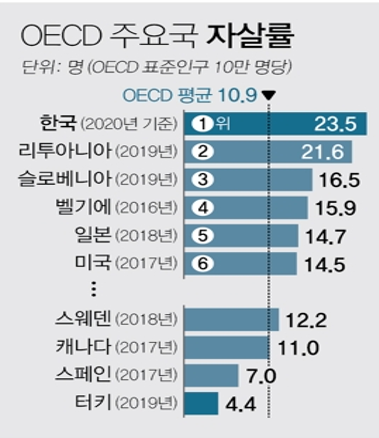
\includegraphics[height = 6cm, width = \linewidth]{picture2.png}
        \caption{OECD 국가별 자살률 비교}
        \label{fig:pic1}
        \endminipage\hfill
        \minipage{0.44\textwidth}
        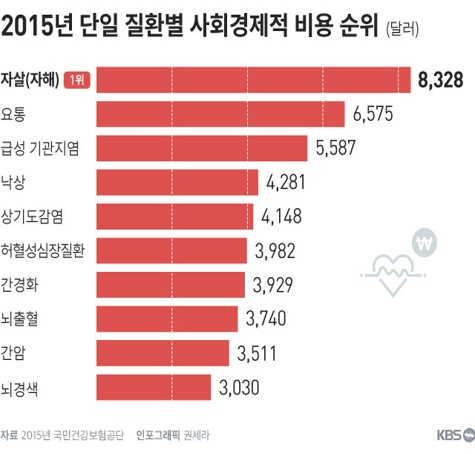
\includegraphics[height = 6cm, width = \linewidth]{picture1.jpg}
        \caption{질환별 사회경제적비용}
        \label{fig:pic2}
        \endminipage\hfill
    
    \end{figure}
    \begin{figure}[h!]
        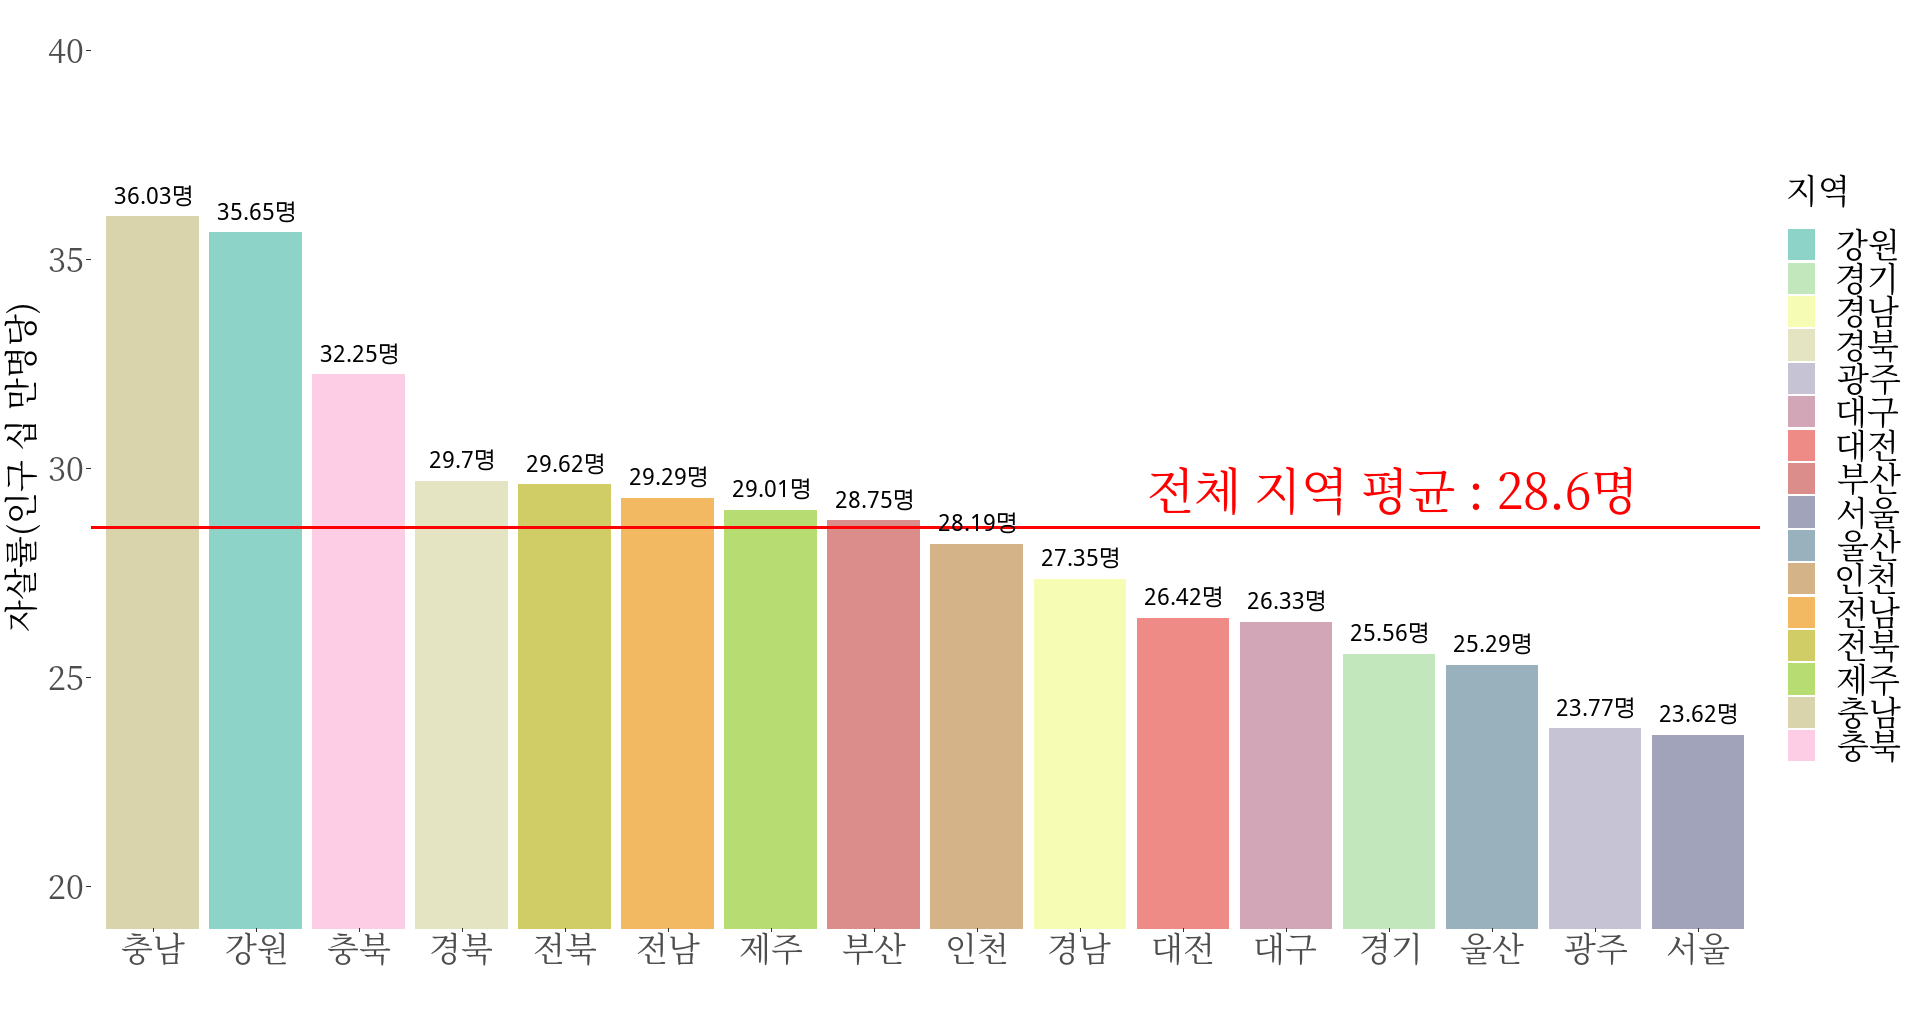
\includegraphics[width = 1\textwidth]{picture3.png}
        \caption{2011년 - 2020년 지역별 평균 자살률(인구 십 만명당)}
        \label{fig:pic3}
      \end{figure}

    2020년 기준 한국의 인구 십 만명당 자살률은 23.5명으로 OECD 평균인 10.9명에 비해 굉장히 높은 수치를 보이고 있다.(그림 1) 
    이와 같이 높은 자살률은 개인의 슬픔과 고통에 국한된 것이 아니라, 실질적으로도 사회경제적으로 큰 손실을 안긴다.(그림 2)
    
    이와 같은 배경 속에서, 국내의 높은 자살률을 줄이기 위해서는 어떠한 요소에 대한 검토가 필요한지 판단하고자 본 연구를 수행하였다. 
    즉, 자살률과 상관성이 높은 요소를 판별하는 것을 통해서 자살률을 줄이기 위해서 가장 먼저 조절되어야 할 필요성이 있는 요소를 
    찾고자 한다. 자살률과 관계가 있는 변인을 구별 해내기 위해서 각 KOSIS 통계 포털에 등록되어있는 지역별 e-지방지표를 활용한다. 
    위 데이터를 통해서 지역별로 자살률의 차이가 존재하는 것을 확인하였고(그림 3), 지역 간의 변인 비교를 통해서 지역 간의 자살률 차이를 만드는
    변인을 파악하면, 국내 자살률이 타 국가에 비해서 높게 나타나는 변인 또한 추정할 수 있을 것이라 판단했다. 
    
    \section{분석}
    \subsection{선행연구}
    선행연구를 찾아보았을 때 사회경제적 불평등, 개인의 신체적/정신적 문제, 환경적 문제 등이 대표적으로 언급되었다. \\
    \begin{tcolorbox}
        사회경제적 양극화, 상대적 박탈감 심화등으로 인해 사회적 연대감이 지속적으로 약화되어 우울증·스트레스 등의 정신건강 문제를 야기하였으며, 이로 인한 자살이 지속적으로 증가하고 있다.
        (이용재 \& 김경미, 2018) 자살의 경제학 이론에 의하면 빈곤은 자살의 중요한 원인이 되며, 사회의 물질적 기초를 감안할 때, 자살률의 변화는 경제이론에 의해 예측될 수 있고 경제 변수와 관련된다고 보았다.
        (이용재 \& 김경미, 2018) 자살자 중에서 정신질환을 가지고 있지 않는 사람들이나 정신질환 보유 여부가 불투명한 경우가 더 많다. 그러므로 이들의 자살 원인에 대하여 생활 부적응, 경제적 곤란, 건강 문제 등 다양한 자살 동기에 주목할 필요가 있다.  
        (김기원 \& 김한곤, 2011) 사회 통합 및 복지수준이 자살률에 중요한 영향을 미친다는 사실을 보여주었다. (이민아 \& 강정한, 2014)   
    \end{tcolorbox}
    
    한국생명존중희망재단에서 발간한 `5개년(2013~2017) 전국 자살사망 분석 보고서'에 따르면 정신건강문제, 경제문제, 신체건강문제가 주요한 자살의 원인으로 판별되었다.
    동일한 보고서에서 건강보험료 소득 분위 구간별로 자살발생사망률을 분석했을 때, 소득 수준이 낮을 수록 인구 십 만명당 자살률이 높아지는 것으로 나타났다.(의료급여구간 43.5명,
    소득하위구간 30.0명, 소득중위구간 24.6명, 소득상위구간 19.1명)
    또한 KOSIS 통계포털에 등록되어있는 ``자살충동이유''에 관한 설문조사 데이터를 바탕으로 자살과 관련되어 있는 요소를 추정해보았을 때도 
    경제적 어려움(경제적 요인), 질환에 대한 염려(신체적/정신적 문제) 개인적인 가정의 불화(환경적 문제) 개인적인 감정인 외로움(신체적/정신적 문제) 등이
    자살과 관련되어 있는 것으로 나타났다. (그림 4)
    \begin{figure}[!ht]
        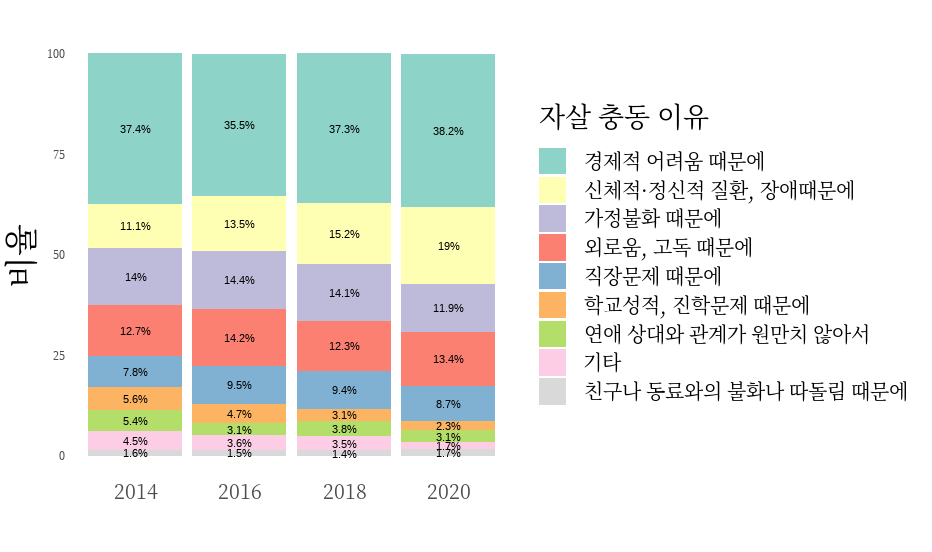
\includegraphics[height = 6.3cm, width = 0.7\textwidth]{picture4.png}
        \caption{자살 충동 이유}
        \label{fig:pic4}
      \end{figure}
    
    \subsection{데이터}
    \begin{figure}[!ht]
        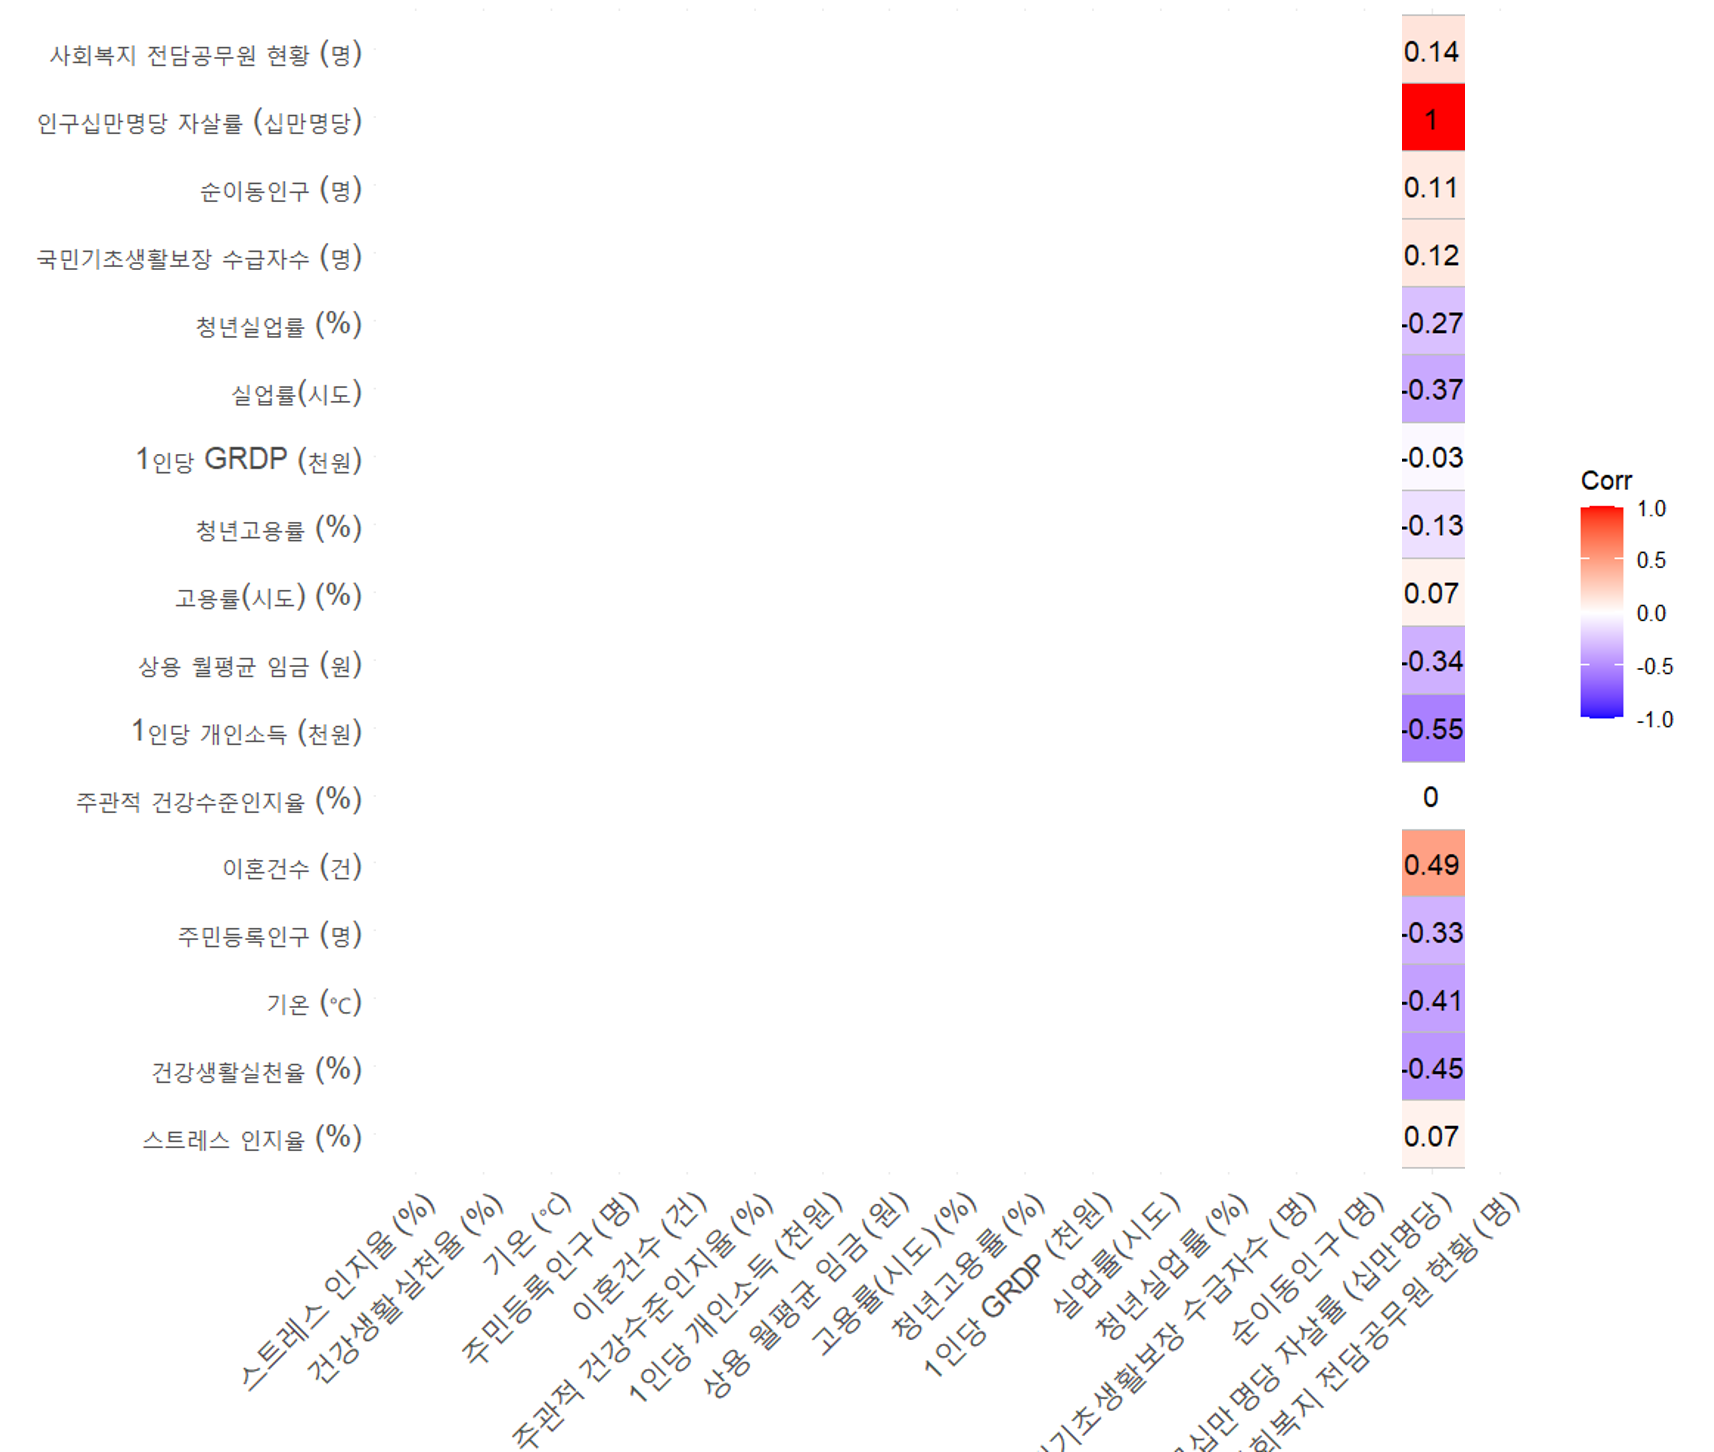
\includegraphics[width = 0.8\textwidth]{picture5.png}
        \caption{15개 변수와 자살률 상관계수 분석}
        \label{fig:pic5}
      \end{figure}
    앞서 살펴본 선행연구와 데이터를 바탕으로 지역별 e-지방지표에서 2011년 - 2020년의 10년간 데이터 중 자살률을 제외한 뒤 각 데이터를
    4가지 범주(경제적요인, 사회적요인, 개인적요인, 환경적요인)로 구분하였다. 이후 각 범주별로 3개 이상의 변인을 선택해 총 15개의 변인에 대해 상관계수 분석을 실시하였다. 
    4가지 범주별로 상관계수가 높은 변인을 1개씩(이혼건수\footnote{주어진 데이터 내의 주민등록 인구 수로 나누어서 1인당 이혼 건수를 이용}, 건강생활실천률,기온, 1인당 개인소득) 선별하였다.(그림 5) 마지막으로, 각 지역의 특성을
    대표할 수 있을 것이라 판단한 ``주민등록인구수''까지 포함하여 총 5개의 변인에 대해서 자살률과의 상관관계 분석을 실시하였다. 
    \\
    선정한 5개 변인과 자살률의 2011년 ~ 2020년 10개년 통합 상관 관계 분석과 함께 2011년 ~ 2020년의 각 연도별로 개별 변인과 자살률의 상관관계 분석을 실시하였다. 
    상관관계 분석에 있어서는 선형회귀를 통해서 상관관계의 방향(음 혹은 양)을 판단하고, $R^{2}$\footnote{$R^{2}$는, 독립변수가 종속변수를 어느 정도로 설명할 수 있는지를 수치화한 지표이며 [0,1]의 값을 가진다. 0인 경우에는 
    독립변수가 종속변수를 전혀 설명하지 못하고 있음 나타내고, 1의 경우에는 독립변수가 종속변수를 완벽하게 설명함을 나타낸다.} 값을 통해 상관관계의 크기를 수치로 파악하였다.  
    \\
    \begin{figure}[!ht]
        \minipage{0.33\textwidth}
        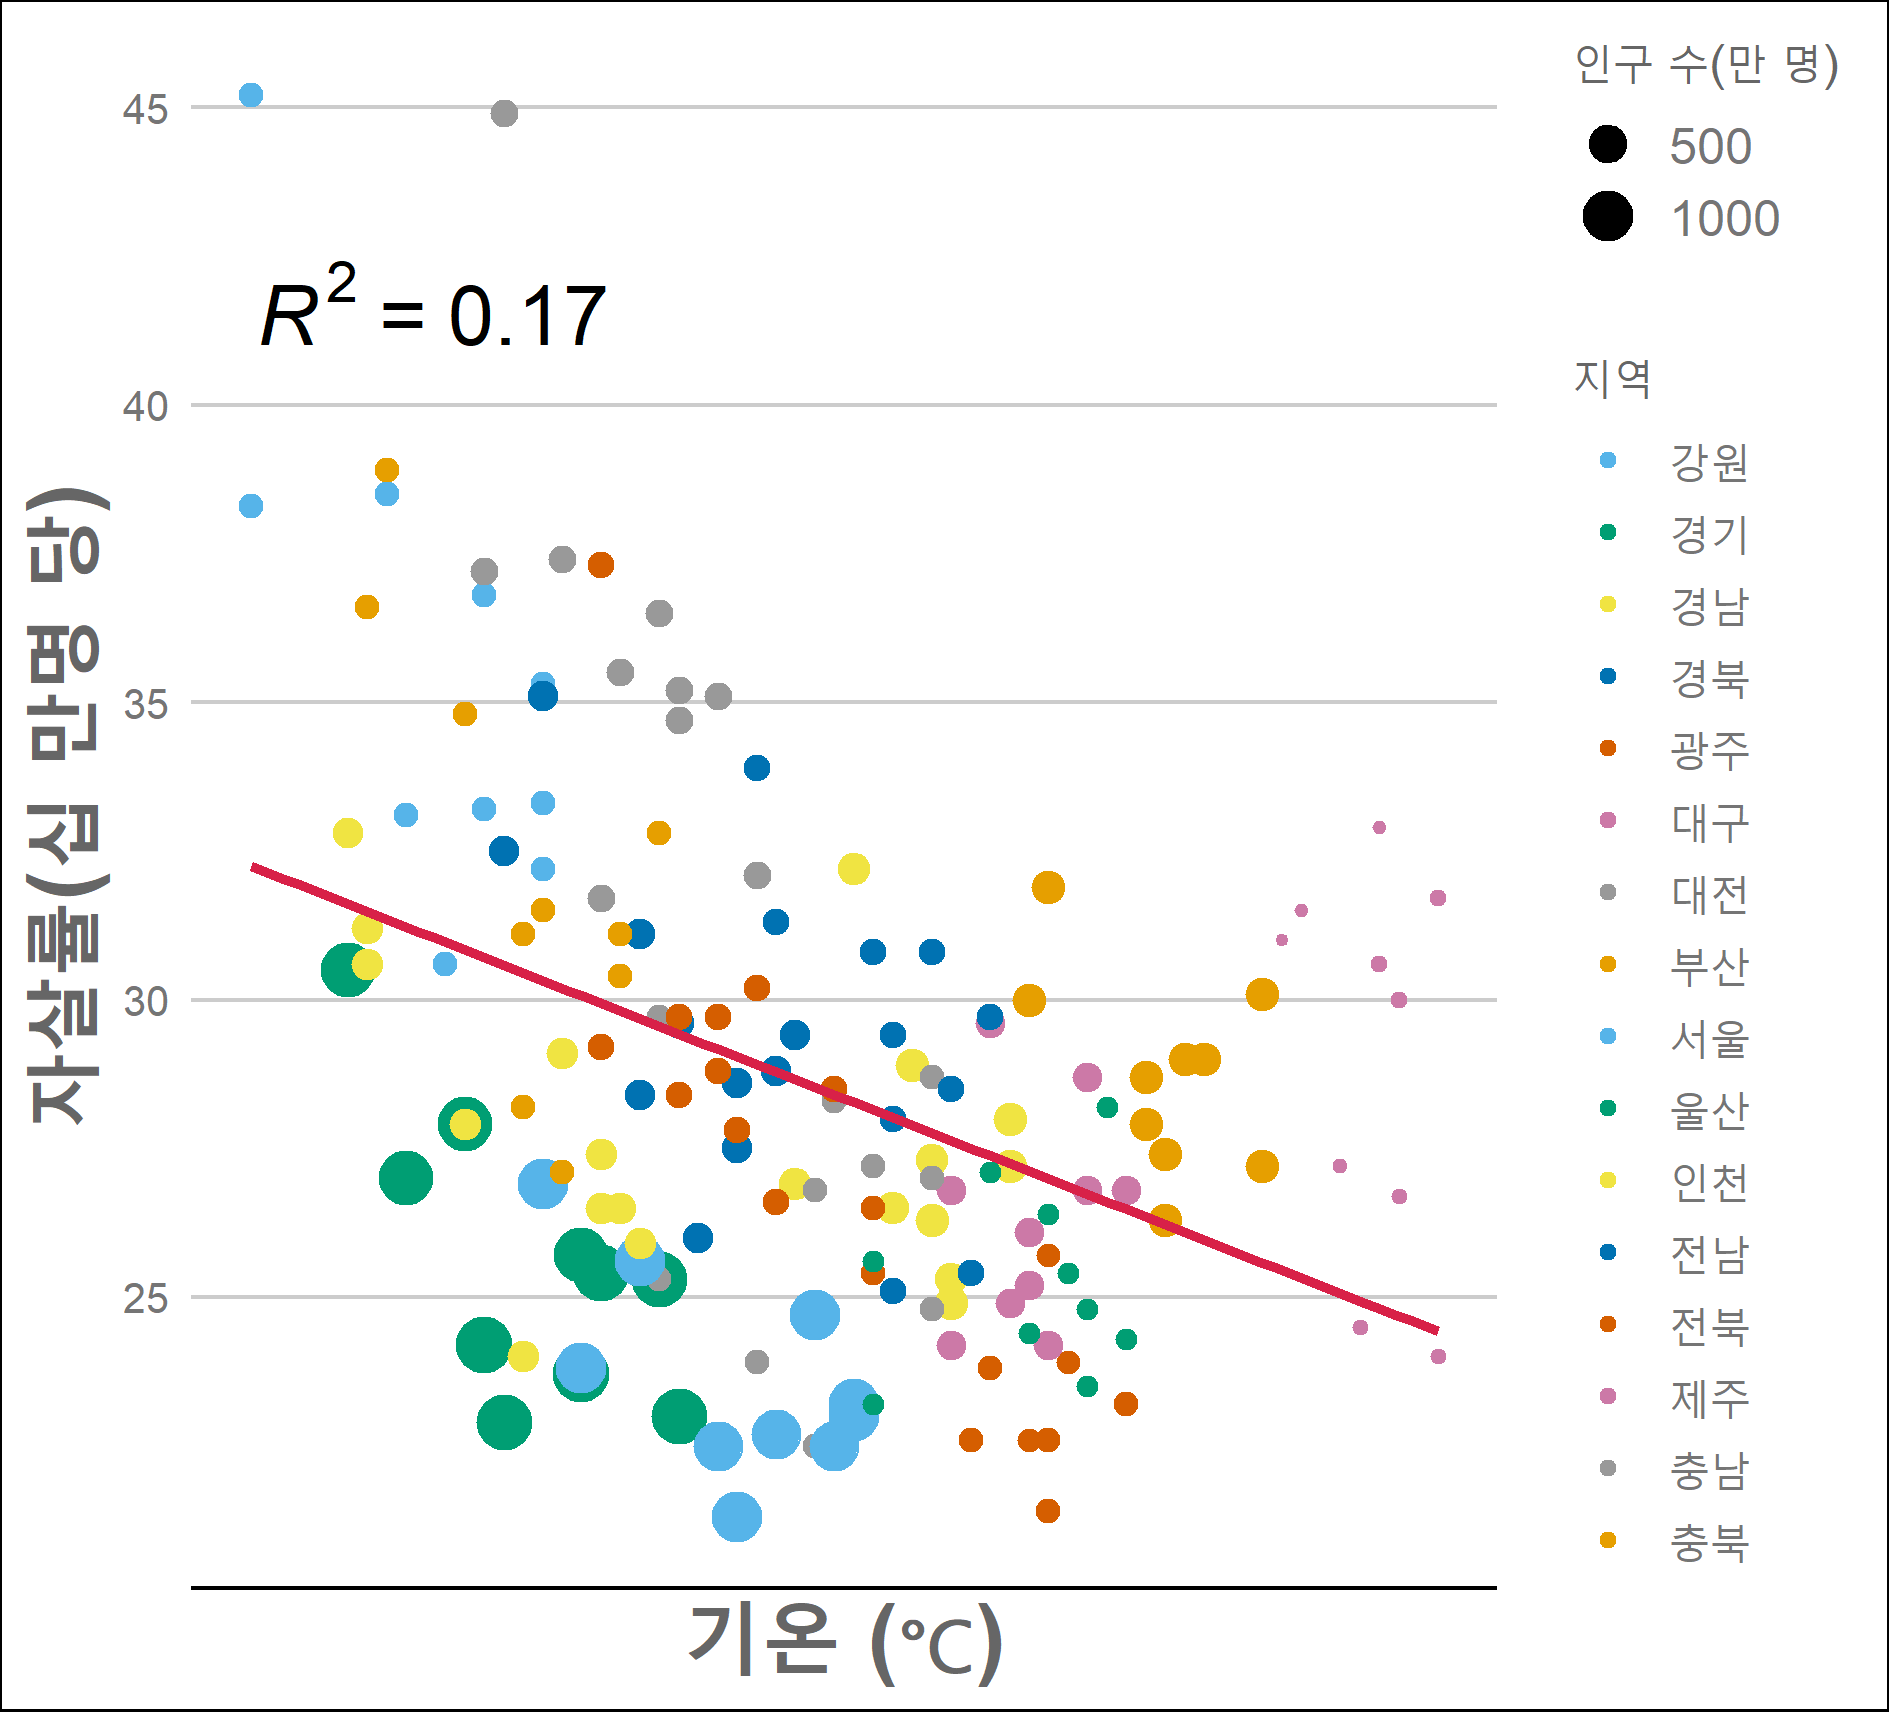
\includegraphics[height = 6cm, width = \linewidth]{c11.png}
        \caption{기온 - 자살률}
        \label{fig:pic11}
        \endminipage\hfill
        \minipage{0.33\textwidth}
        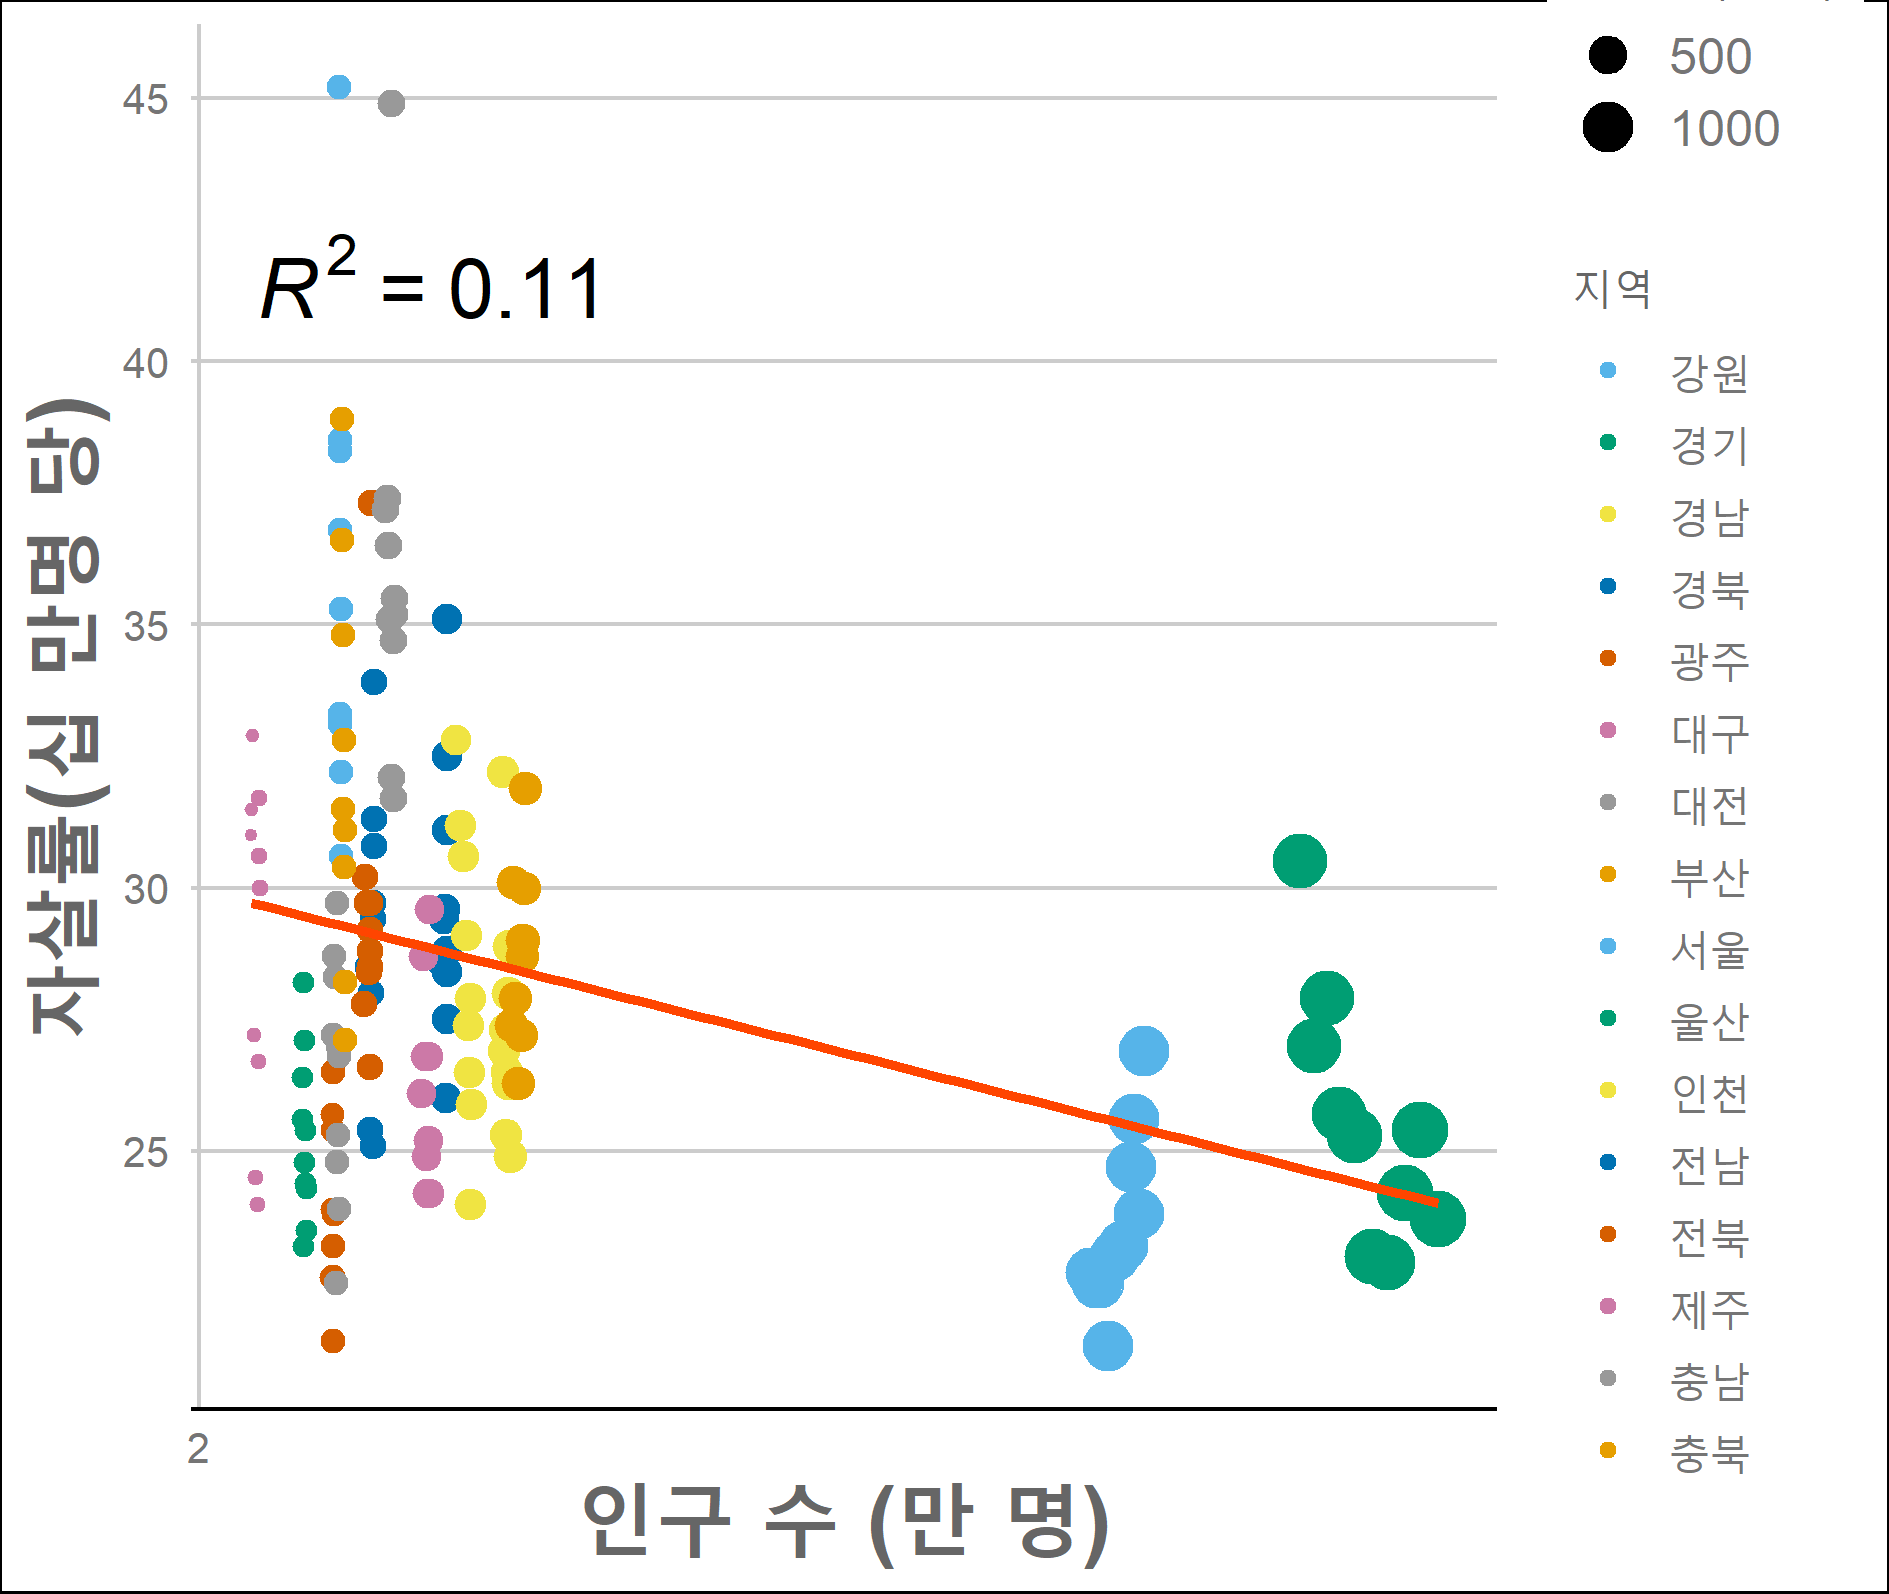
\includegraphics[height = 6cm, width = \linewidth]{c14.png}
        \caption{주민등록인구수 - 자살률}
        \label{fig:pic12}
        \endminipage\hfill
        \minipage{0.33\textwidth}
        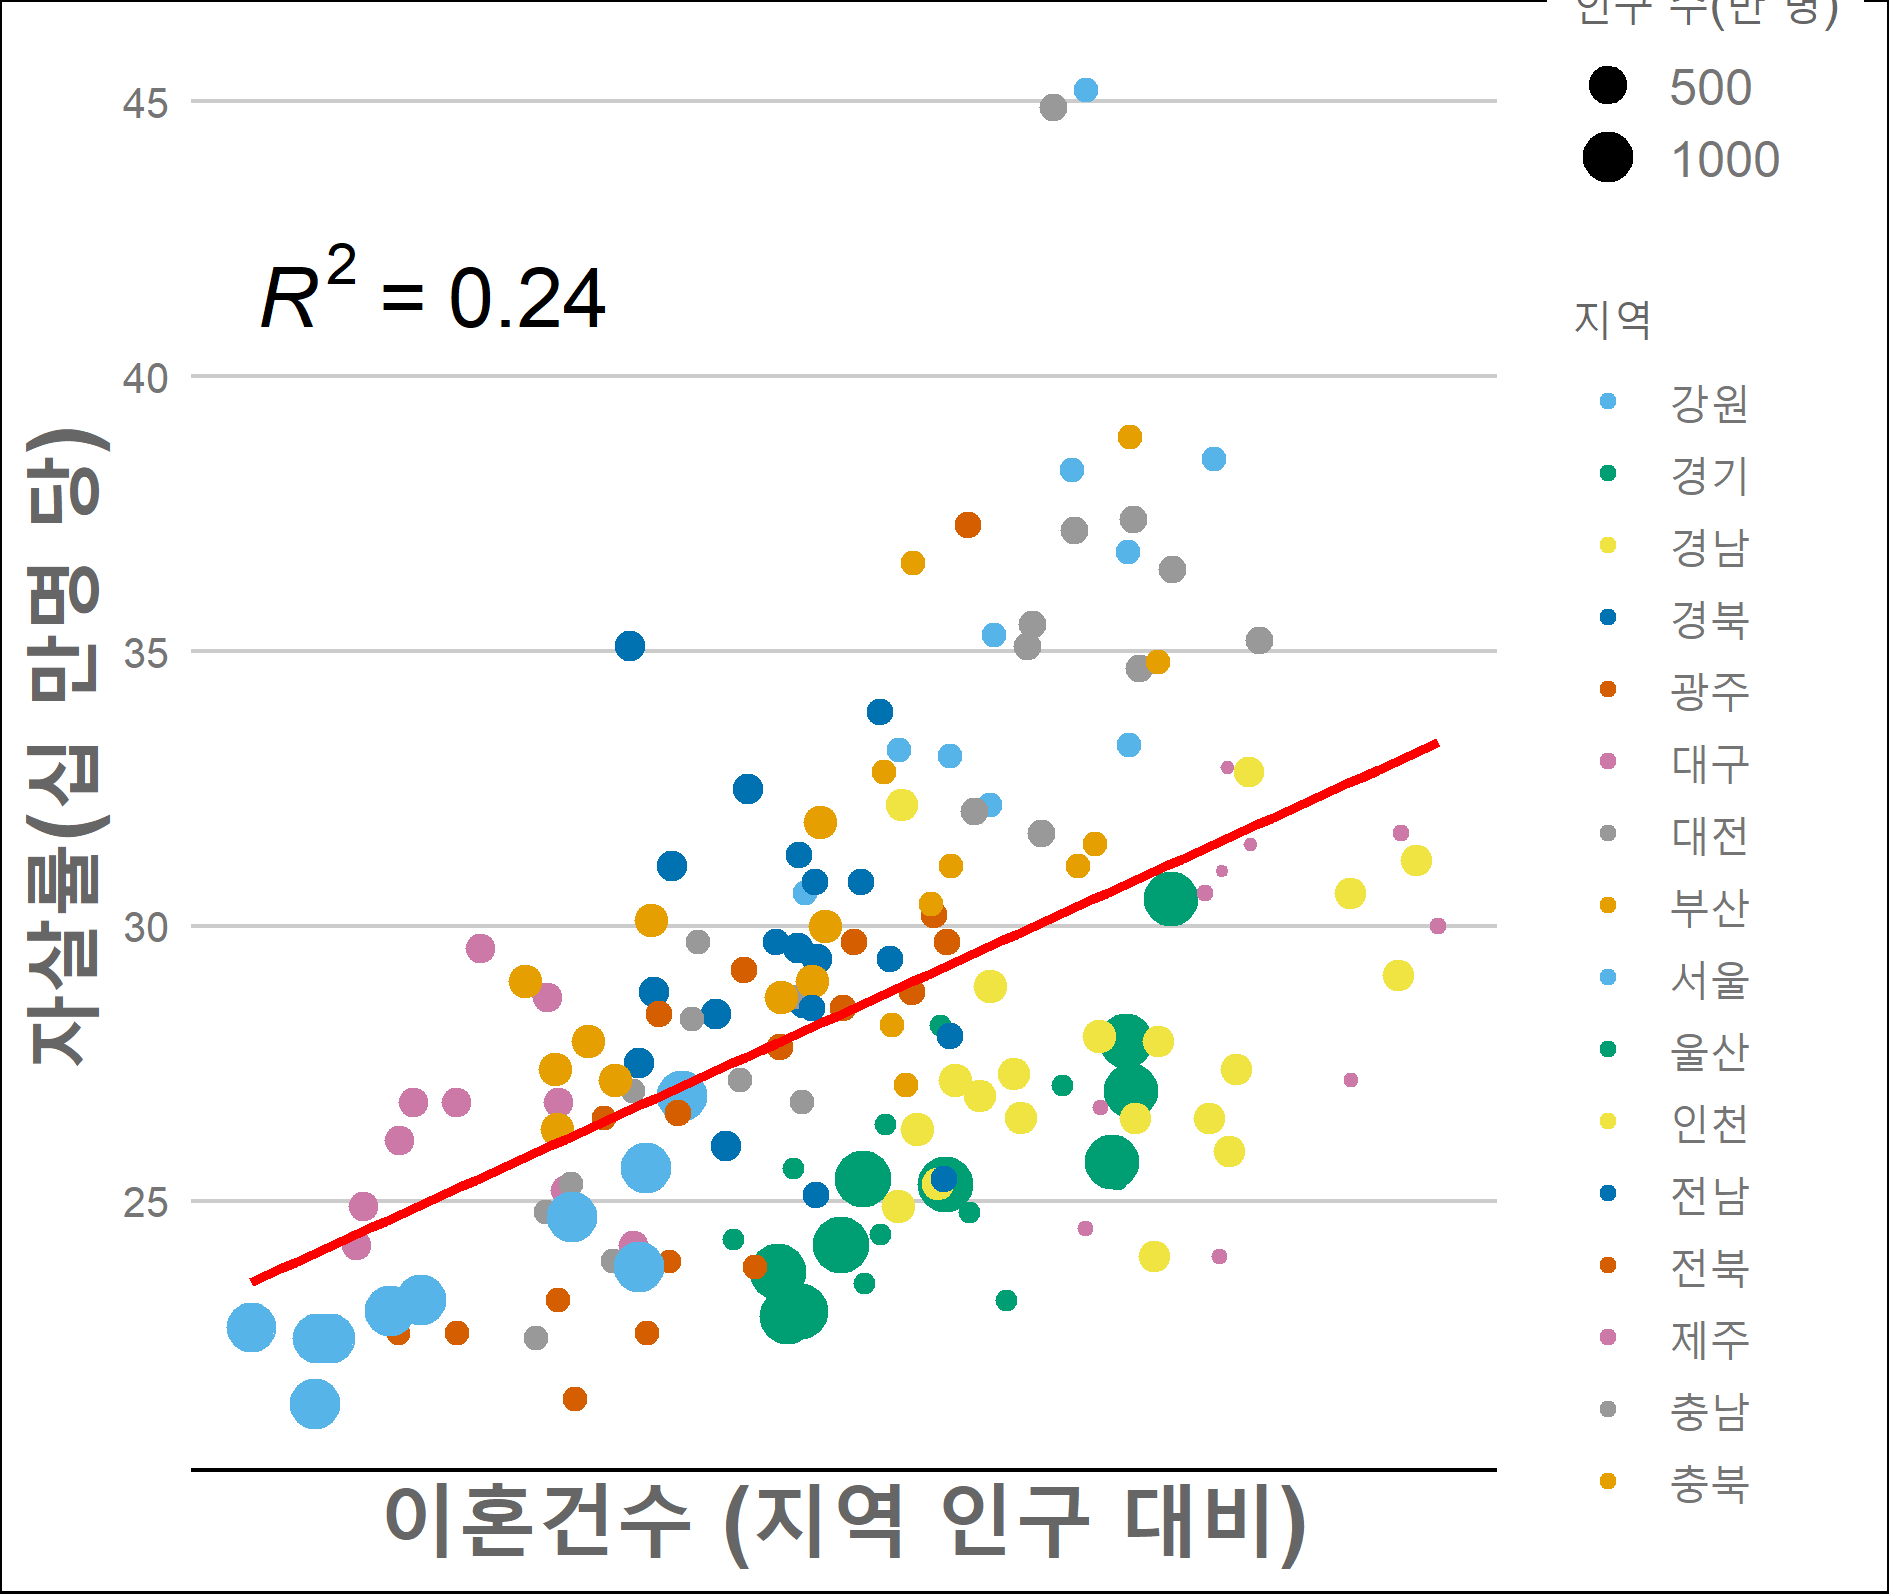
\includegraphics[height = 6cm, width = \linewidth]{c13.png}
        \caption{이혼건수 - 자살률}
        \label{fig:pic13}
        \endminipage\hfill
    
    \end{figure}
    \begin{figure}[!ht]
        \minipage{0.4\textwidth}
        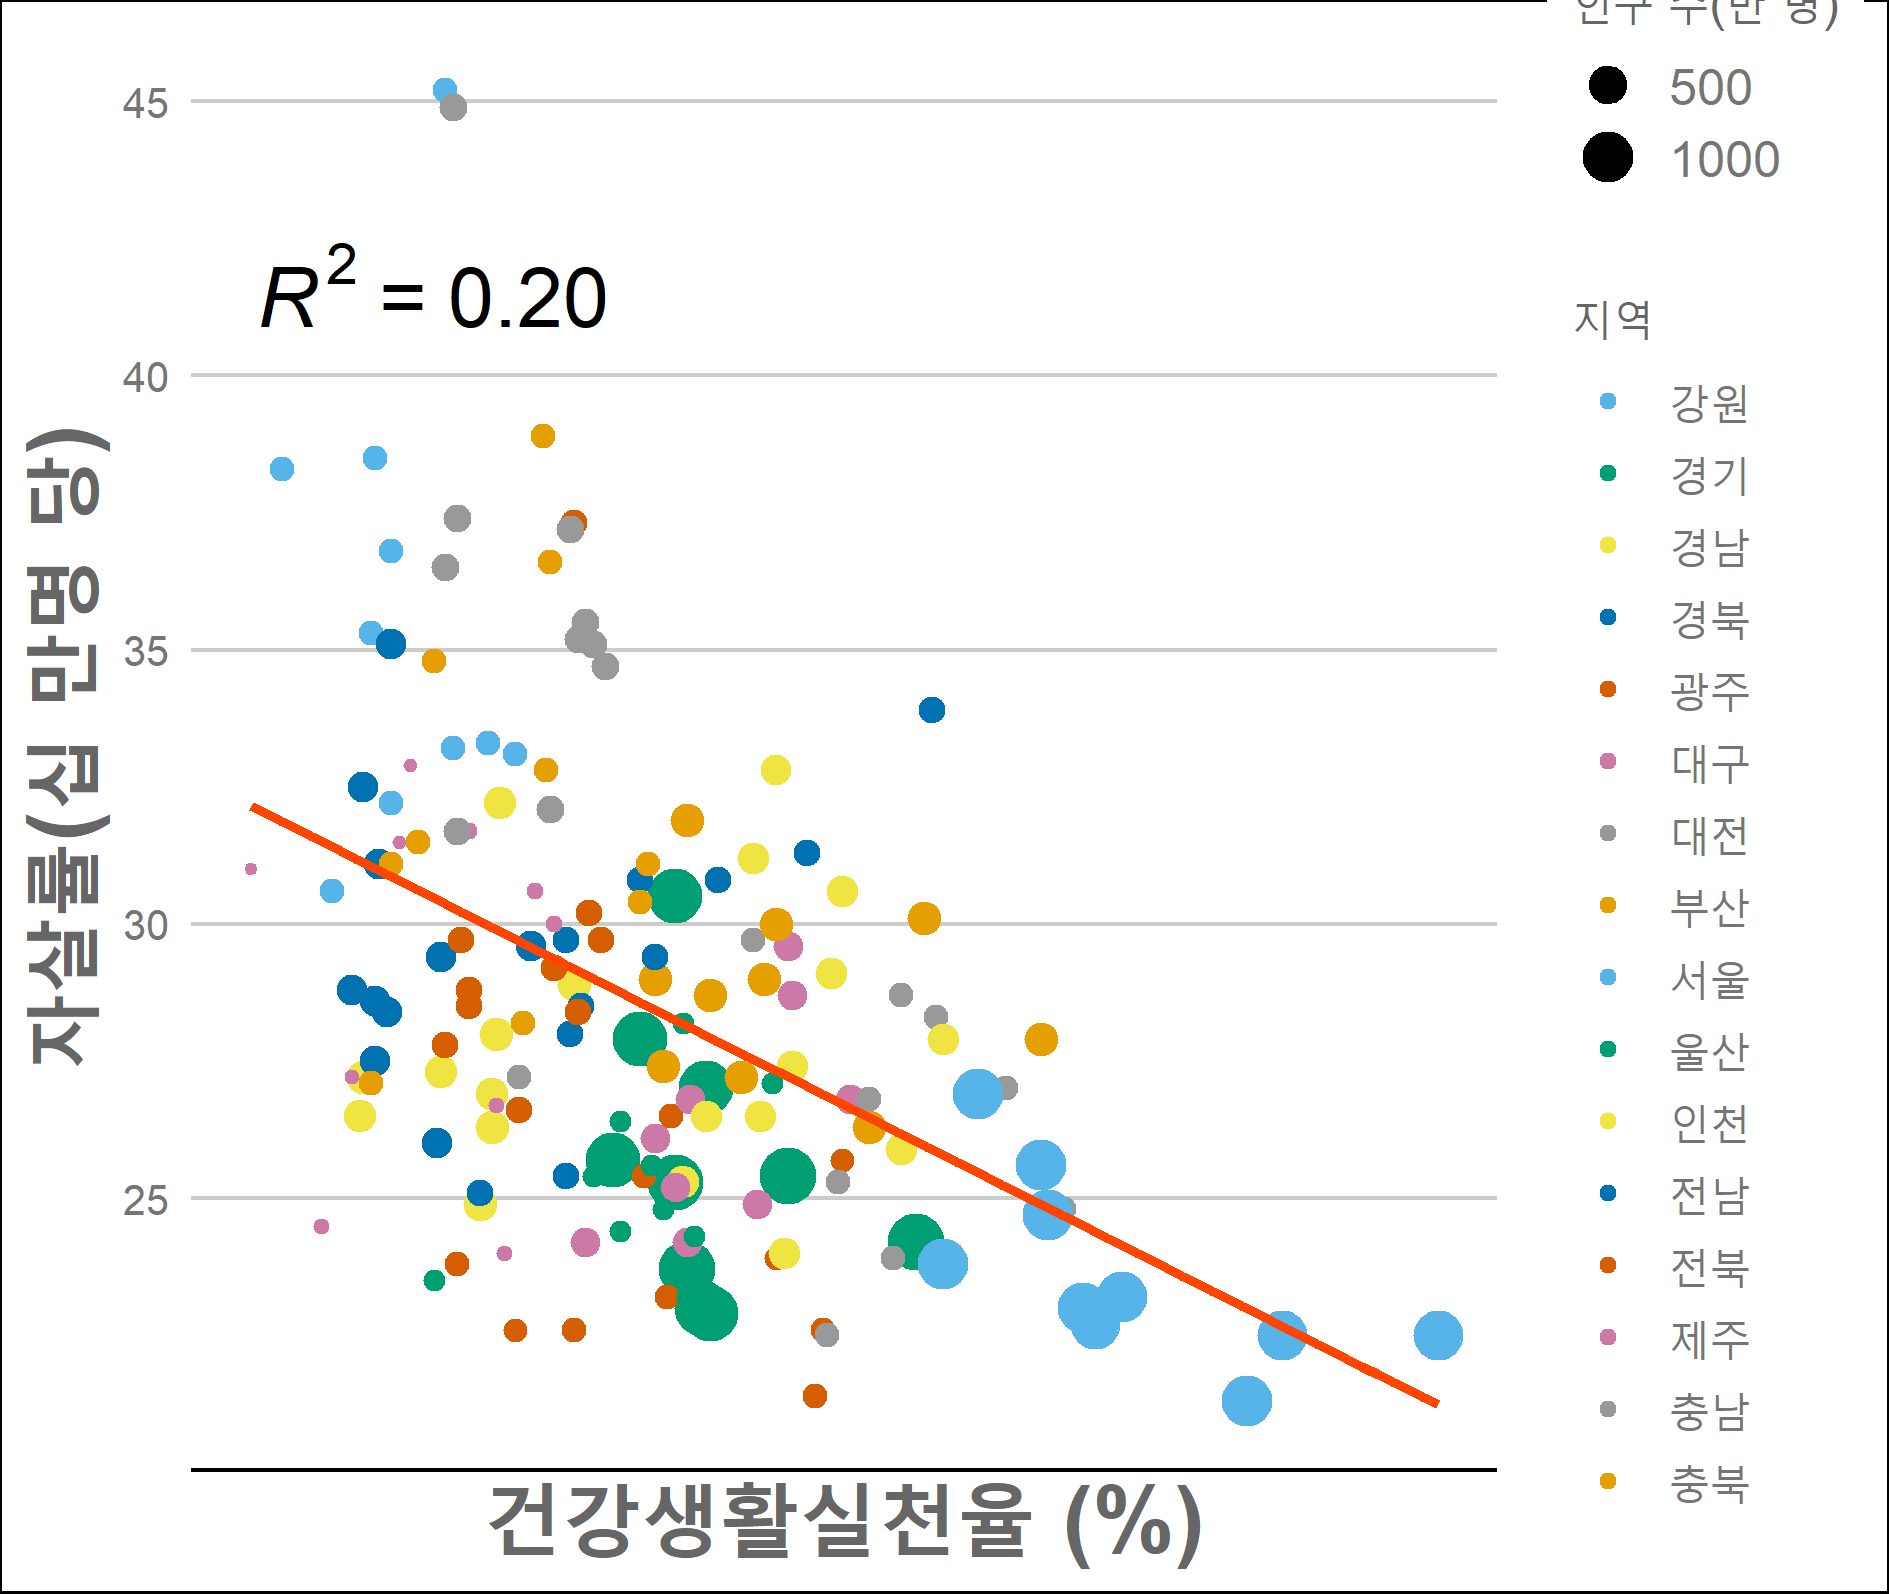
\includegraphics[height = 6cm, width = \linewidth]{c15.png}
        \caption{건강생활실천률 - 자살률}
        \label{fig:pic14}
        \endminipage\hfill
        \minipage{0.4\textwidth}
        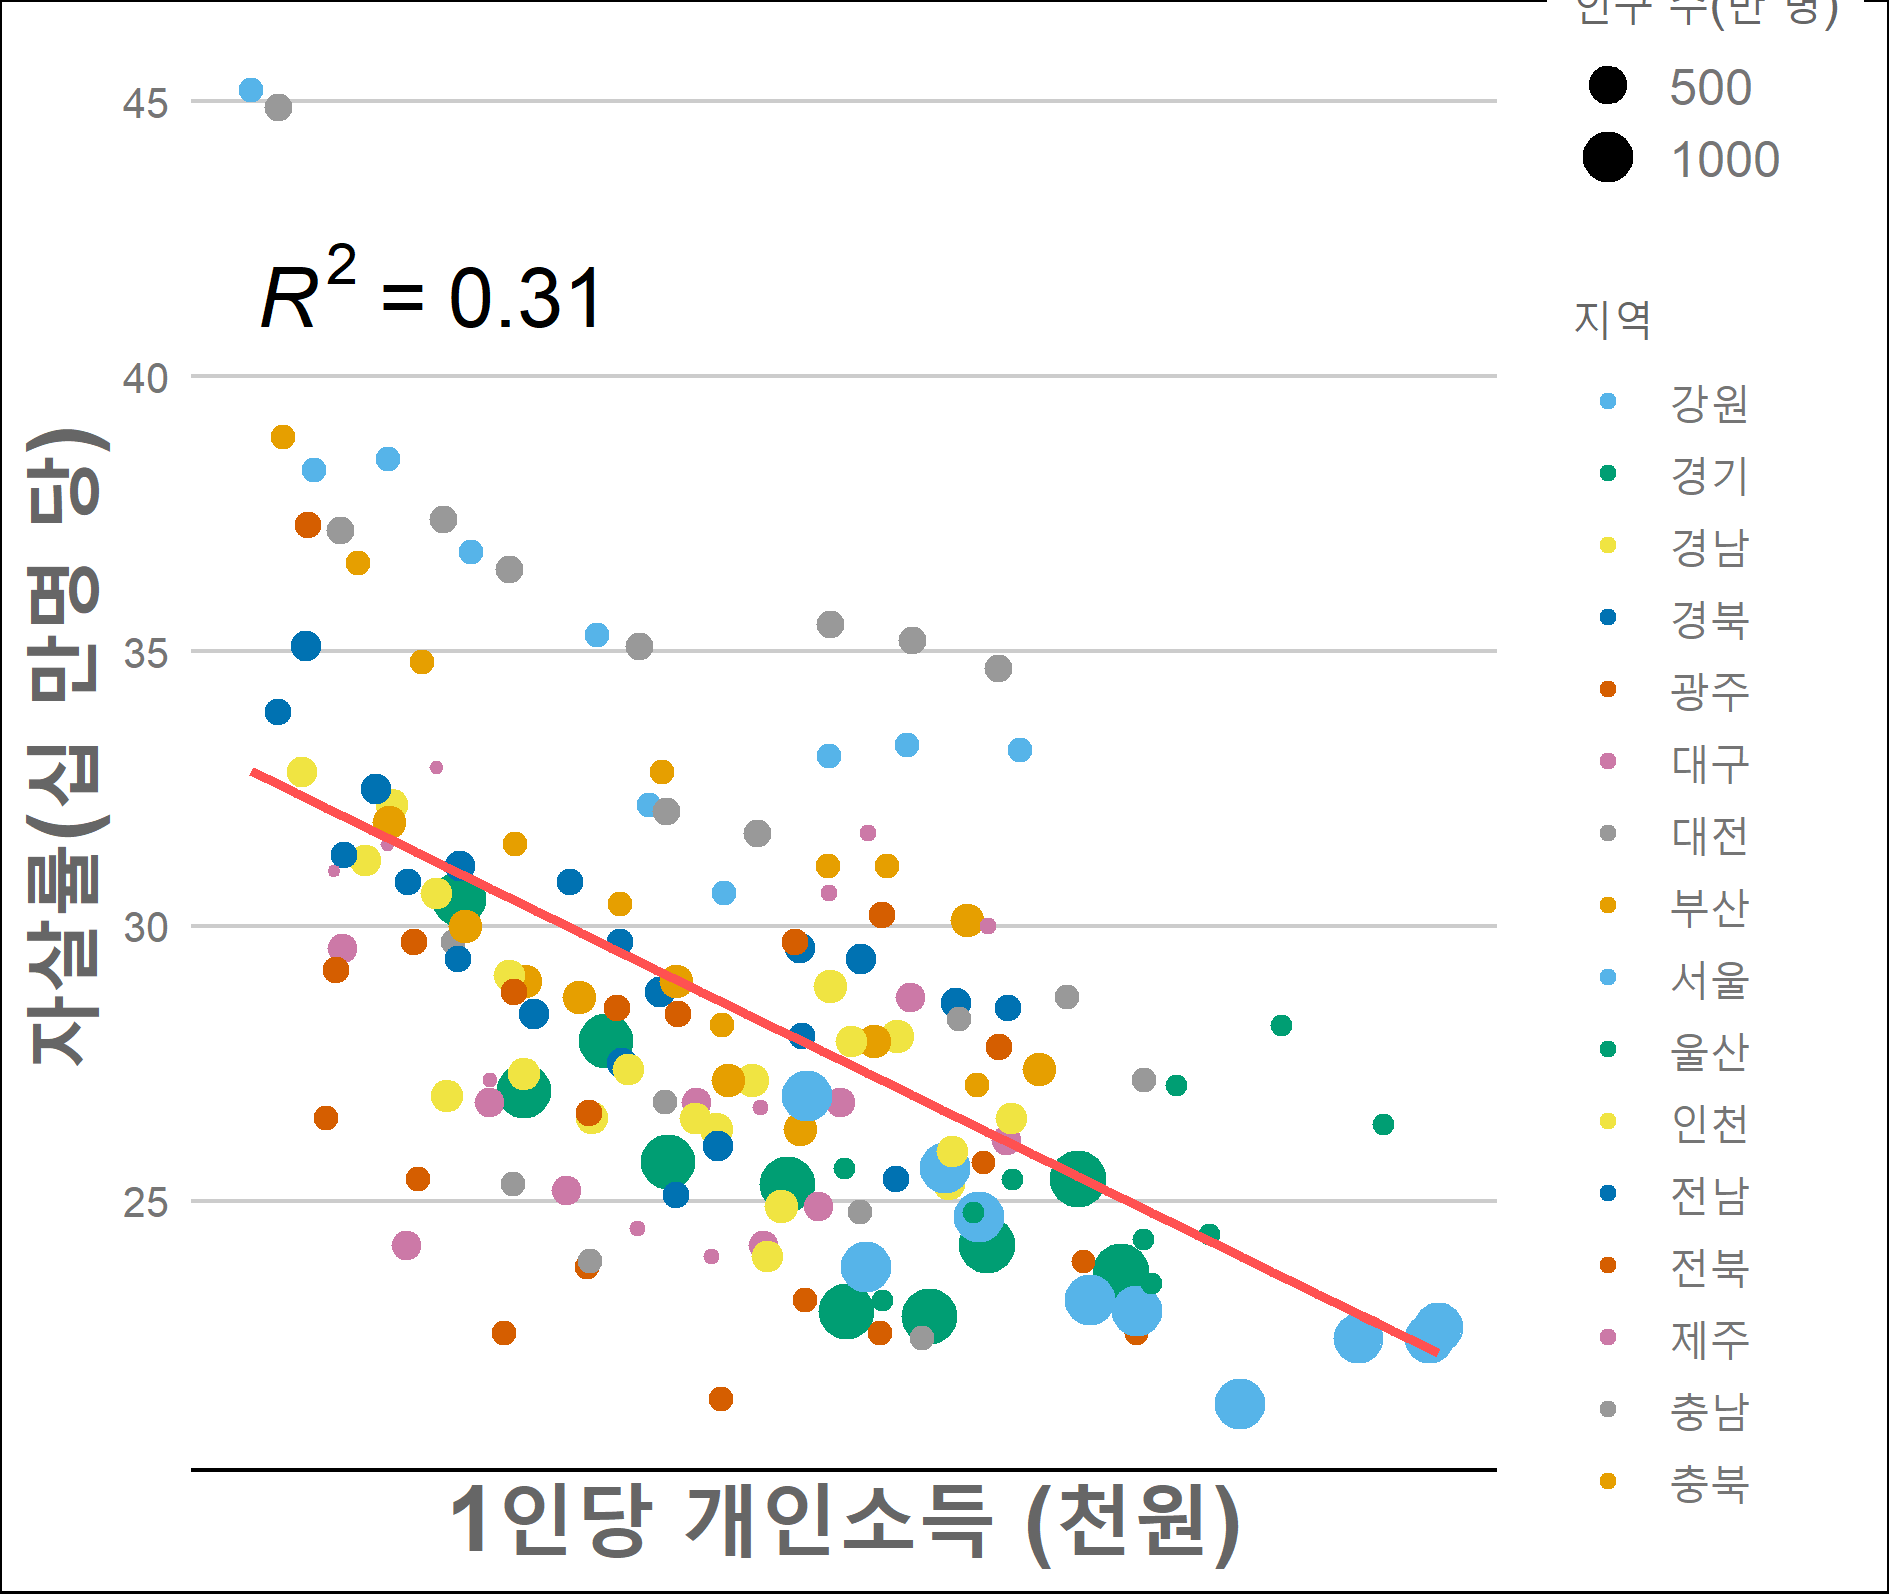
\includegraphics[height = 6cm, width = \linewidth]{c12.png}
        \caption{1인당 개인소득 - 자살률}
        \label{fig:pic15}
        \endminipage\hfill
    \end{figure}
    
    먼저, 개별 연도와 무관하게 각 독립변인과 자살률의 관계를 확인해보고자 하였다. 
    기온(그림 6)과 주민등록인구수(그림 7)은 자살률과 상관성이 낮다고 판단하였다. 기온의 경우, 기온 대비 자살률 수치를 확인해보면
    산점도가 많이 흩어져 나타나는 것을 확인할 수 있었다. 다만, 주민등록인구수의 경우 인구 수가많은 수도권(서울, 경기)과 그 밖의 지방이
    완전히 다른 두 집단을 형성함을 확인할 수 있었고, 자살률 또한 두 집단에서 유의미한 차이를 나타내고 있음을 볼 수 있었다. 
    이혼건수(그림 8)는 앞선 두 변인에 비해서는 자살률과 상대적으로 높은 상관관계를 띔을 확인할 수 있었다. 
    건강생활실천률(그림 9)도 주민등록인구수와 기온에 비교하면 자살률과 높은 상관관계를 띄고 있음을 확인할 수 있었다. 이는 
    스스로 건강생활을 실천하고 있다 느끼는 경우에는 심리적/신체적으로 문제가 적을 가능성이 높이게 자살률과 음의 상관관계를 띄는 것이라 
    생각해볼 수 있다. 마지막으로 개인소득(그림 10)이 다른 4 개의 변인에 비해서 자살률과 가장 높은 상관관계를 띄고 있음을 파악할 수 있었다. 
    선행연구와 자살충동이유 데이터에서 ``경제적문제''가 자살과 관련성이 높은 요인으로 지목되었던 점을 생각해보면, 이러한 높은 상관관계가 
    앞서 살펴본 바와 일치한다는 점을 확인할 수 있었다. 
    \newpage    
    \begin{figure}[!ht]
        \minipage{0.33\textwidth}
        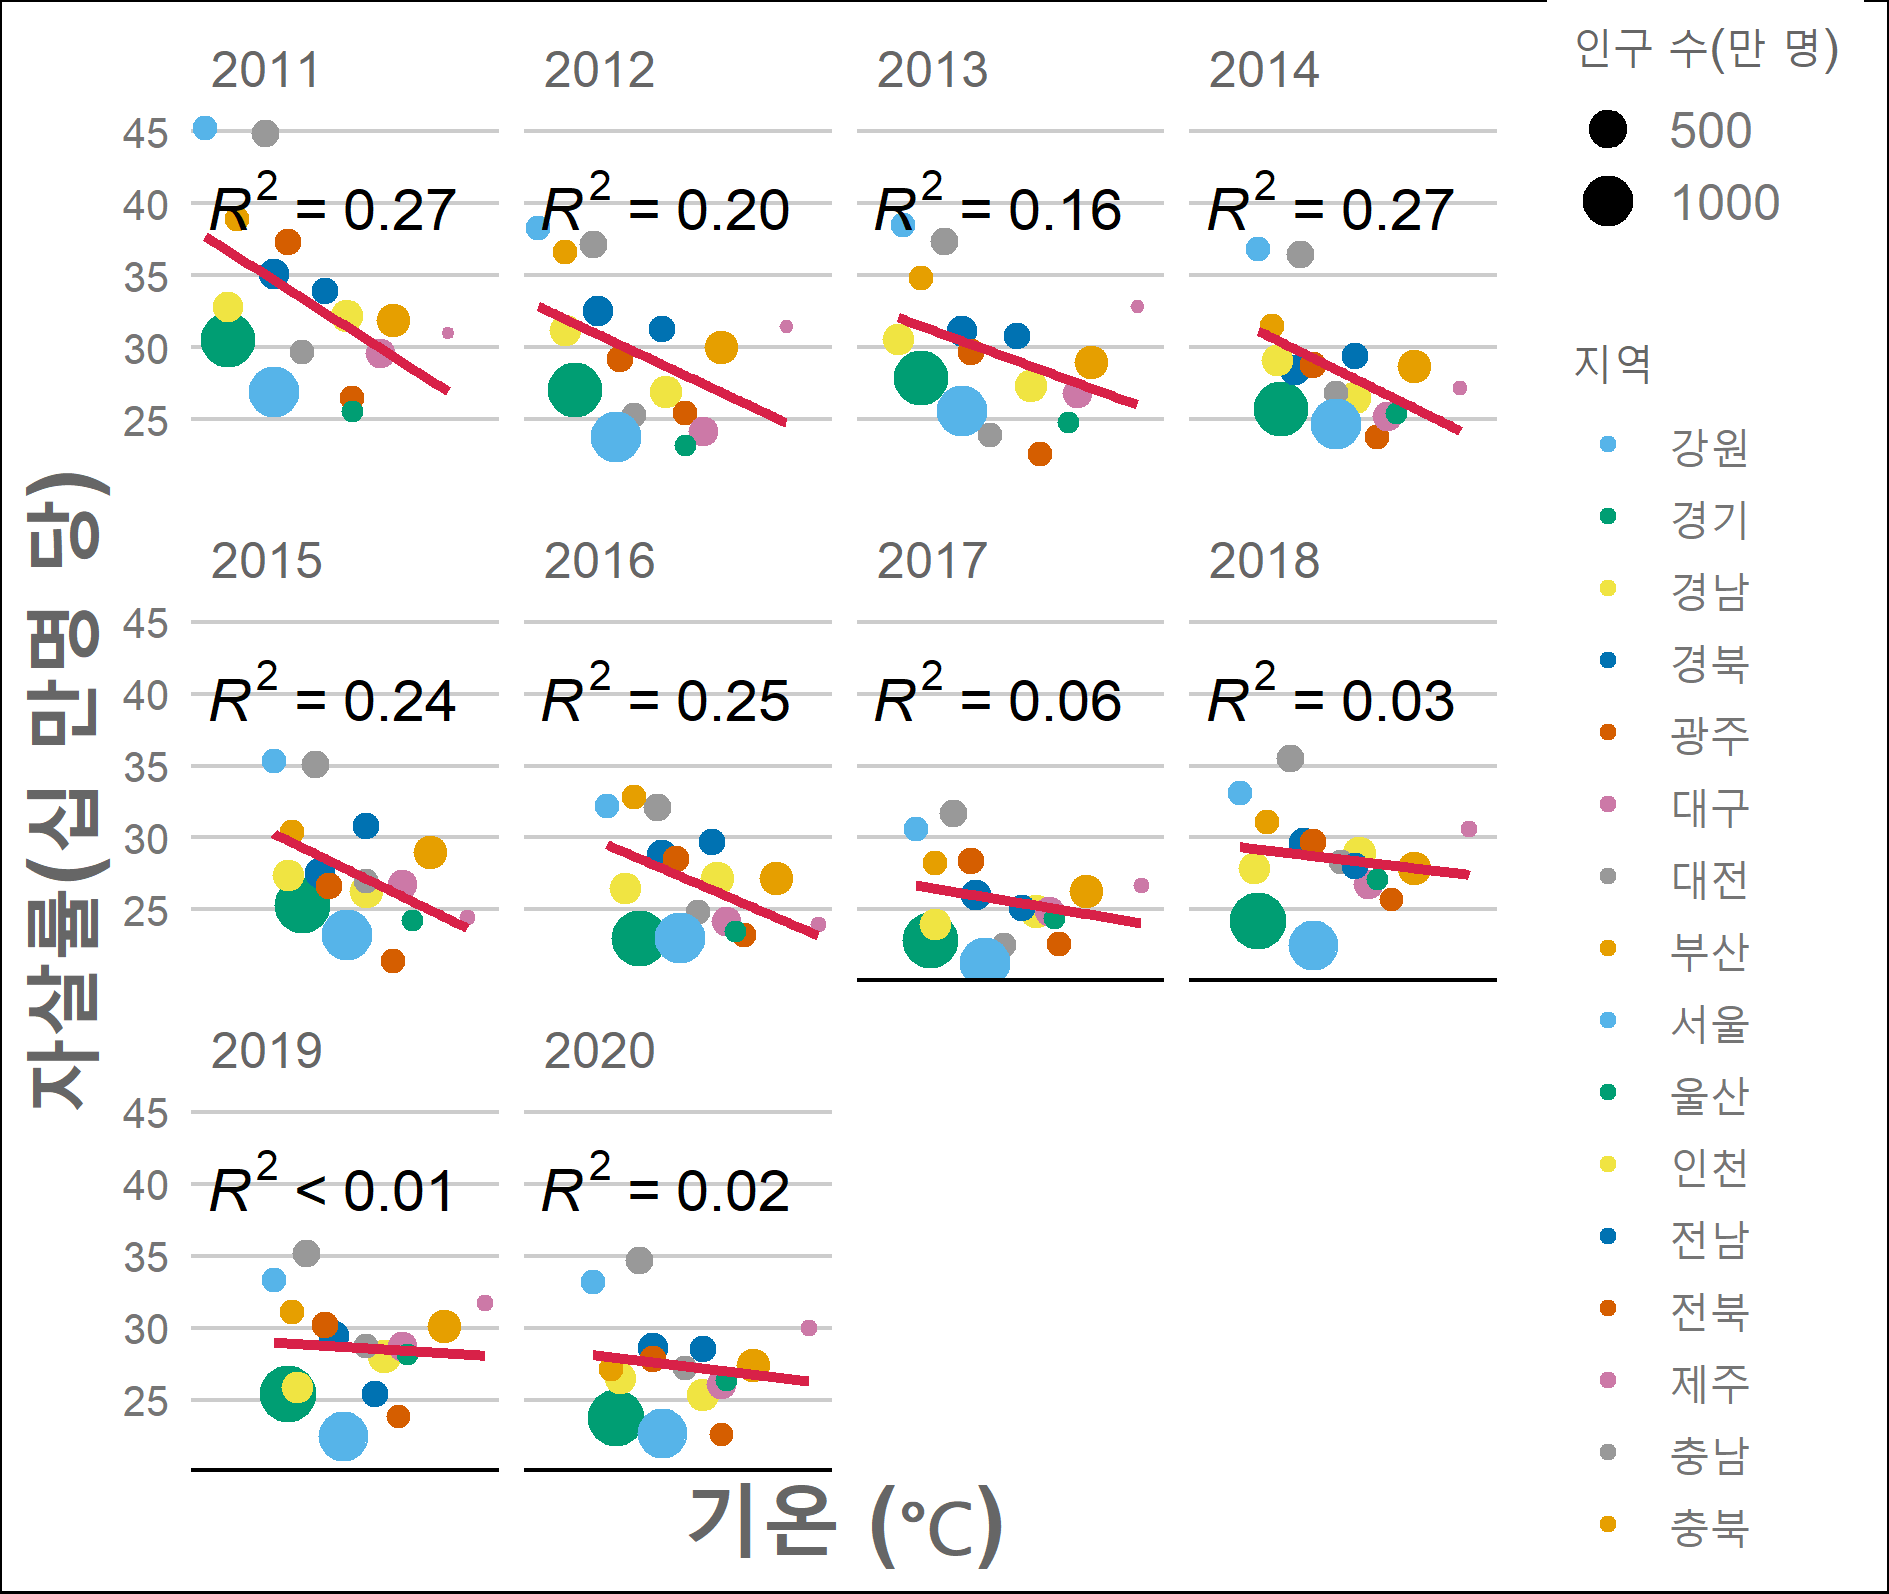
\includegraphics[height = 6cm, width = \linewidth]{c1.png}
        \caption{기온 - 자살률}
        \label{fig:pic111}
        \endminipage\hfill
        \minipage{0.33\textwidth}
        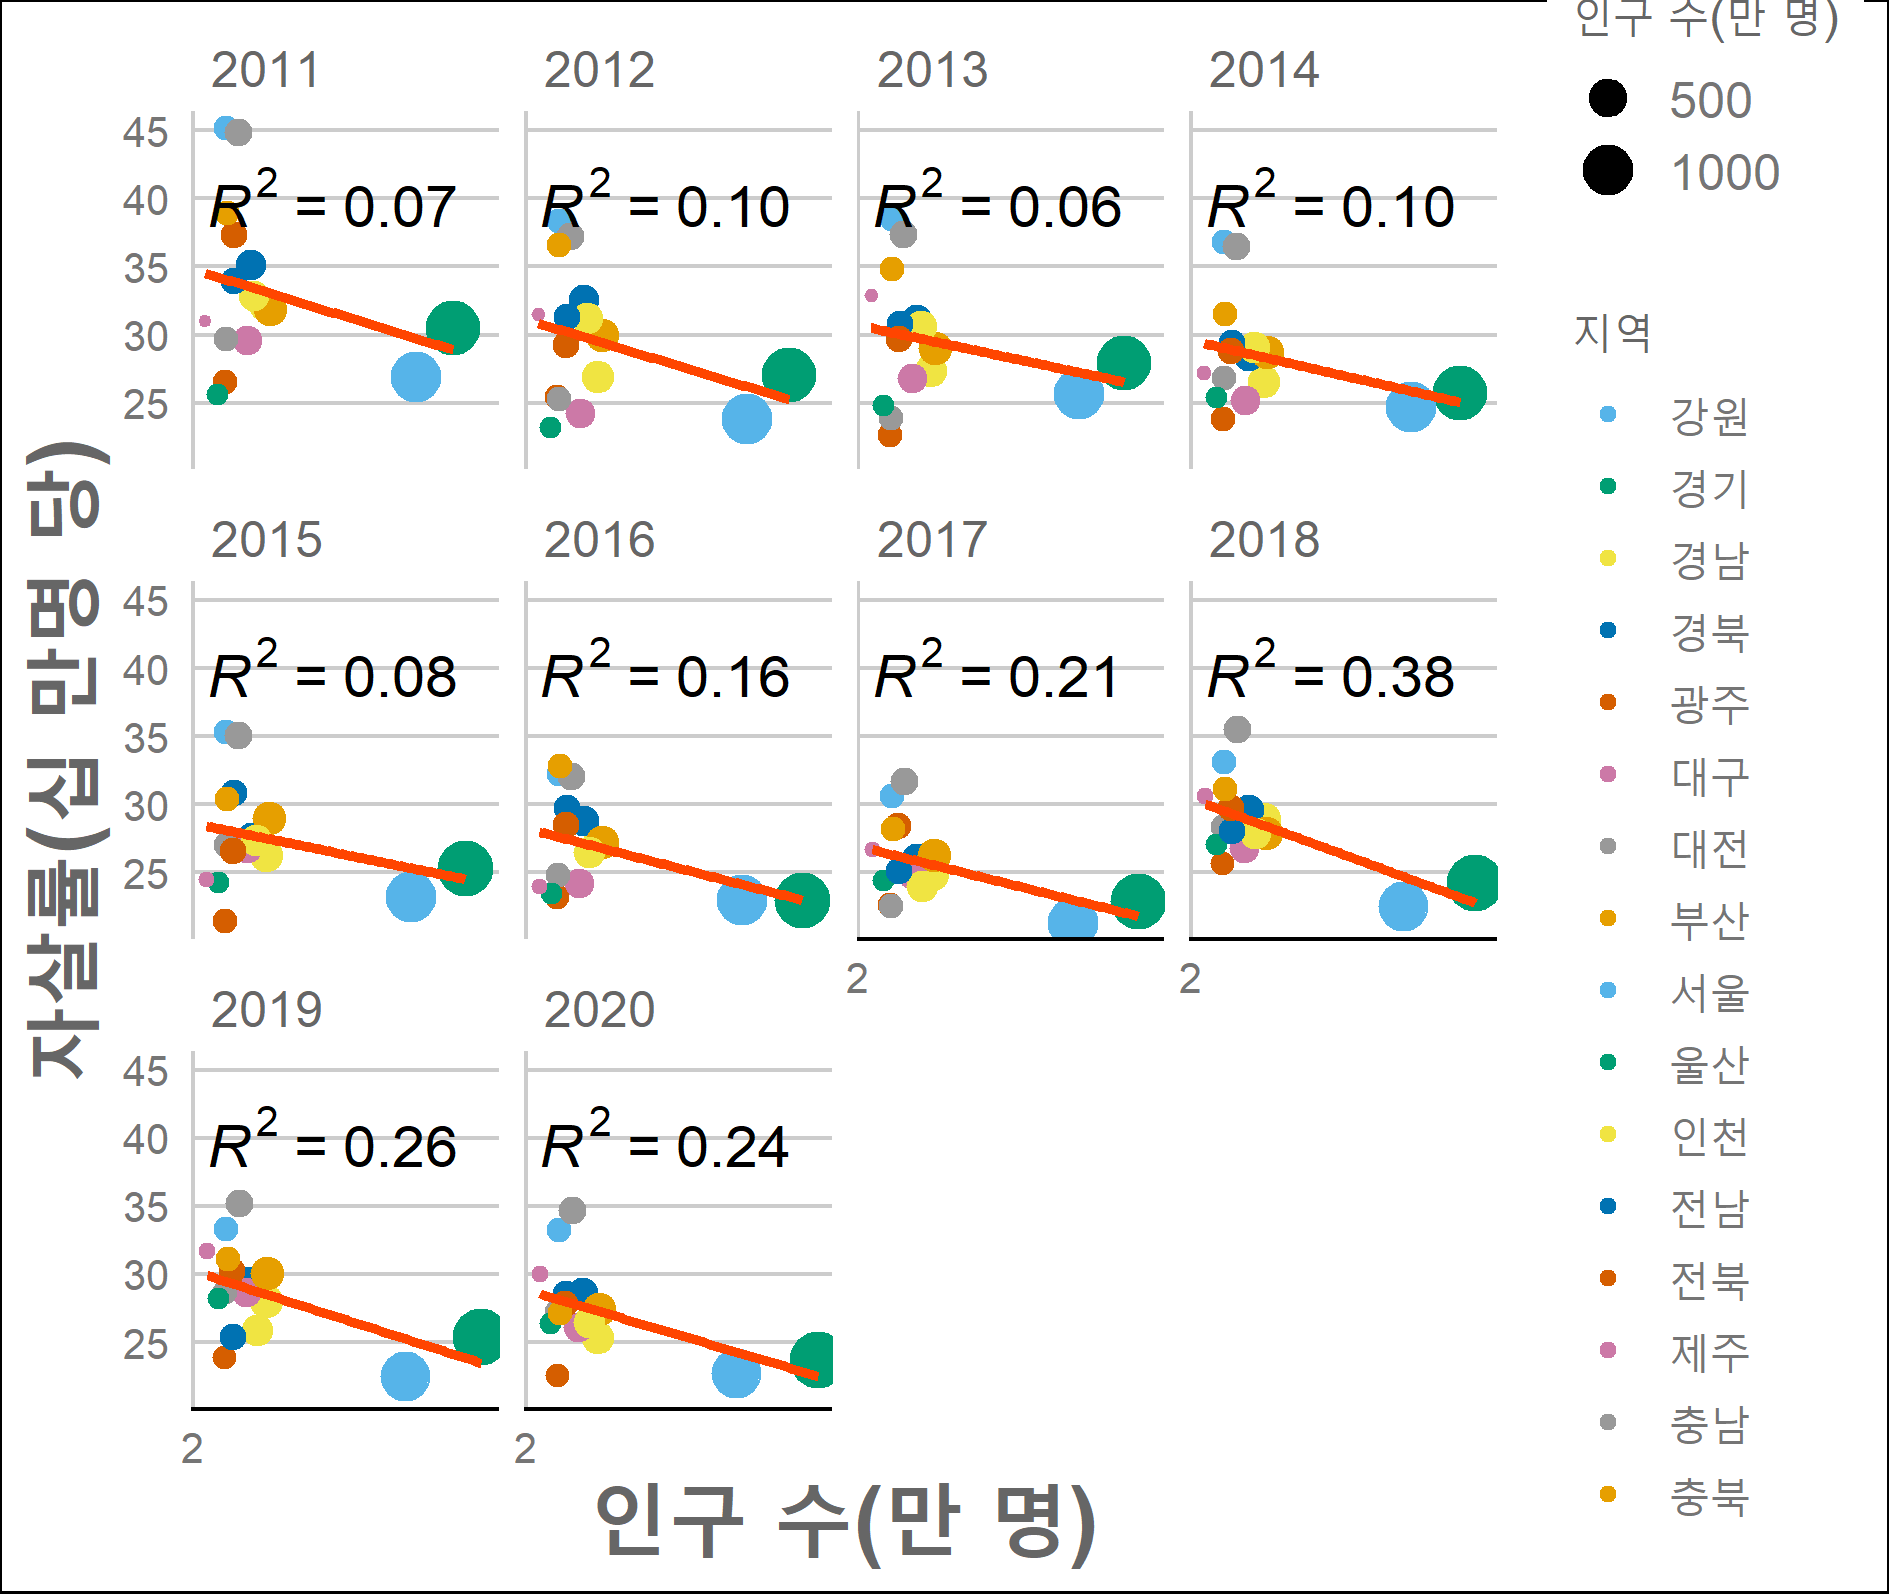
\includegraphics[height = 6cm, width = \linewidth]{c4.png}
        \caption{주민등록인구수 - 자살률}
        \label{fig:pic121}
        \endminipage\hfill
        \minipage{0.33\textwidth}
        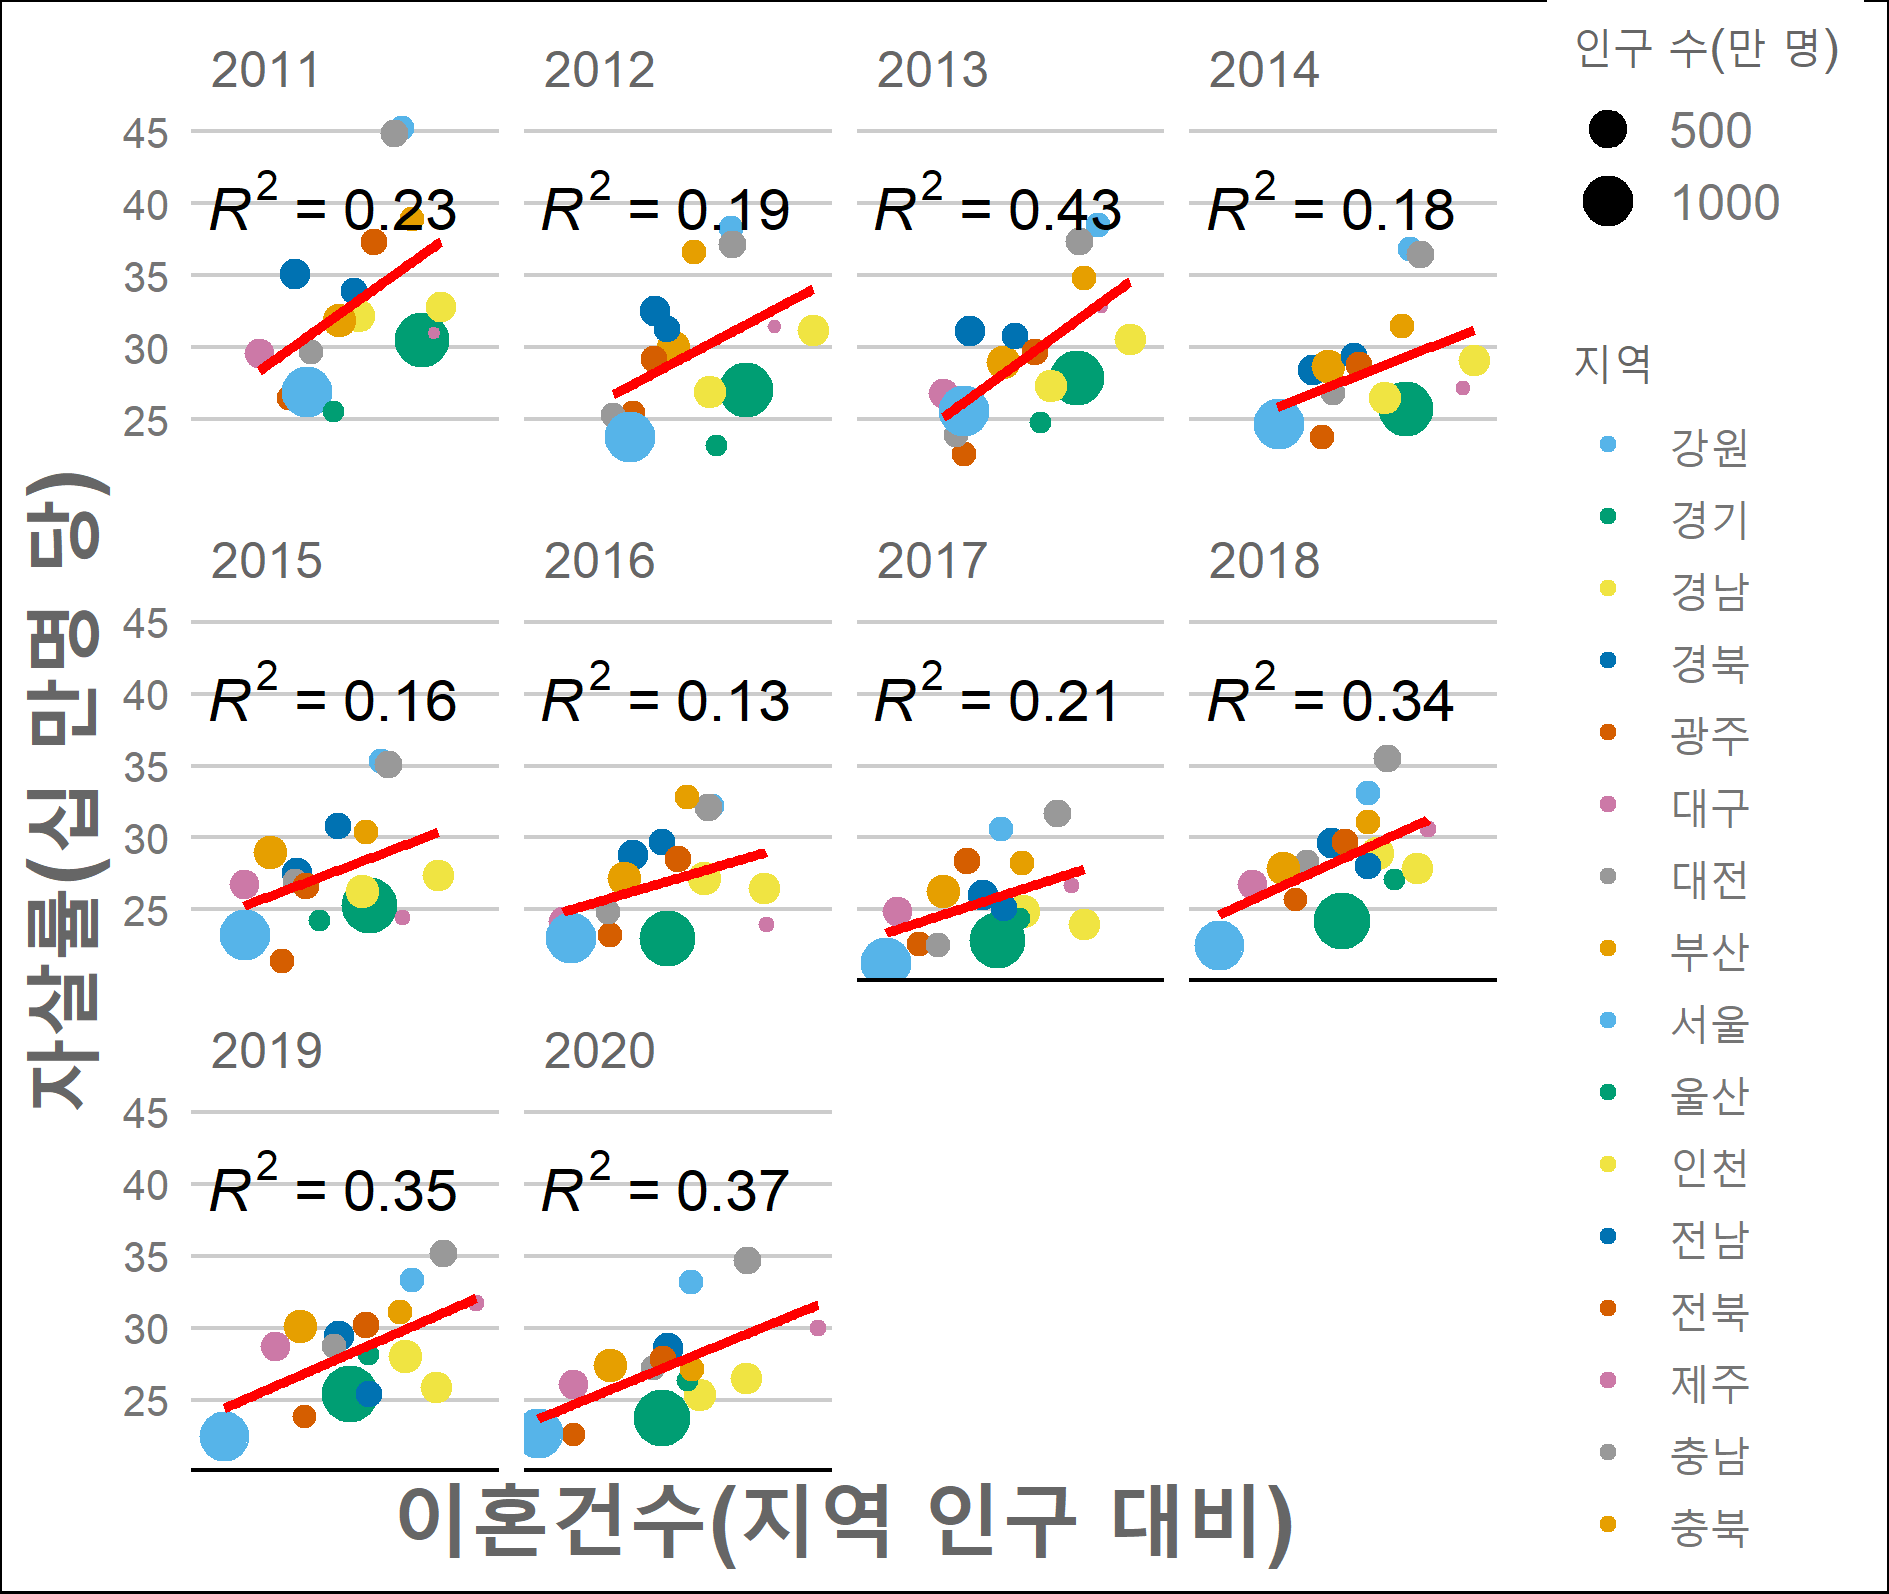
\includegraphics[height = 6cm, width = \linewidth]{c3.png}
        \caption{이혼건수 - 자살률}
        \label{fig:pic131}
        \endminipage\hfill
    
    \end{figure}
    \begin{figure}[!ht]
        \minipage{0.4\textwidth}
        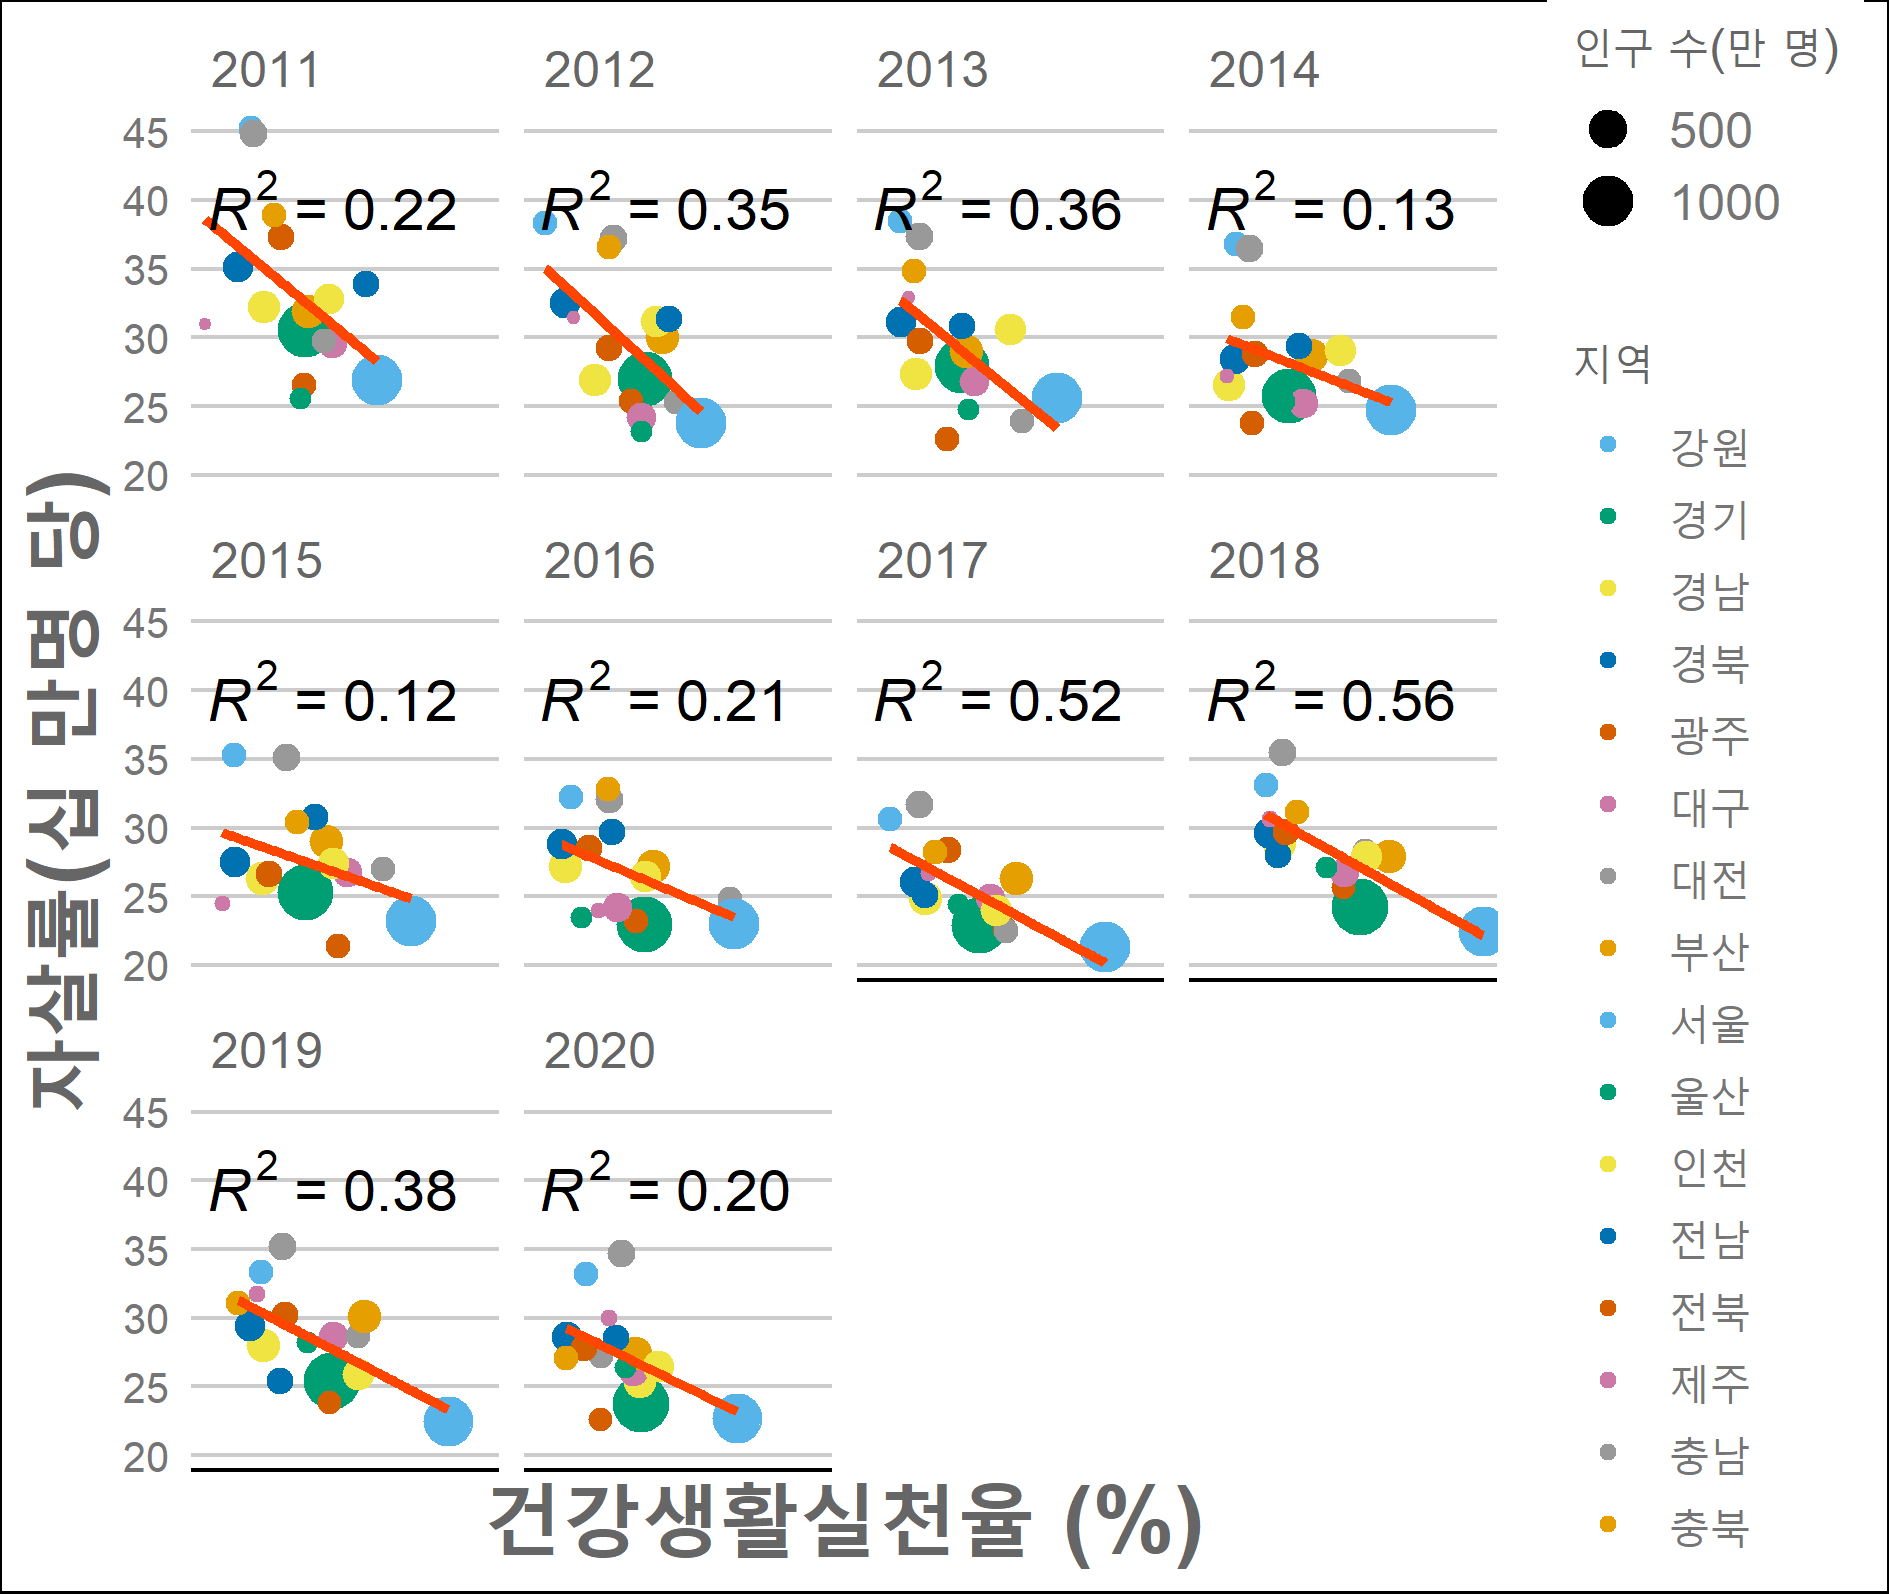
\includegraphics[height = 6cm, width = \linewidth]{c5.png}
        \caption{건강생활실천률 - 자살률}
        \label{fig:pic141}
        \endminipage\hfill
        \minipage{0.4\textwidth}
        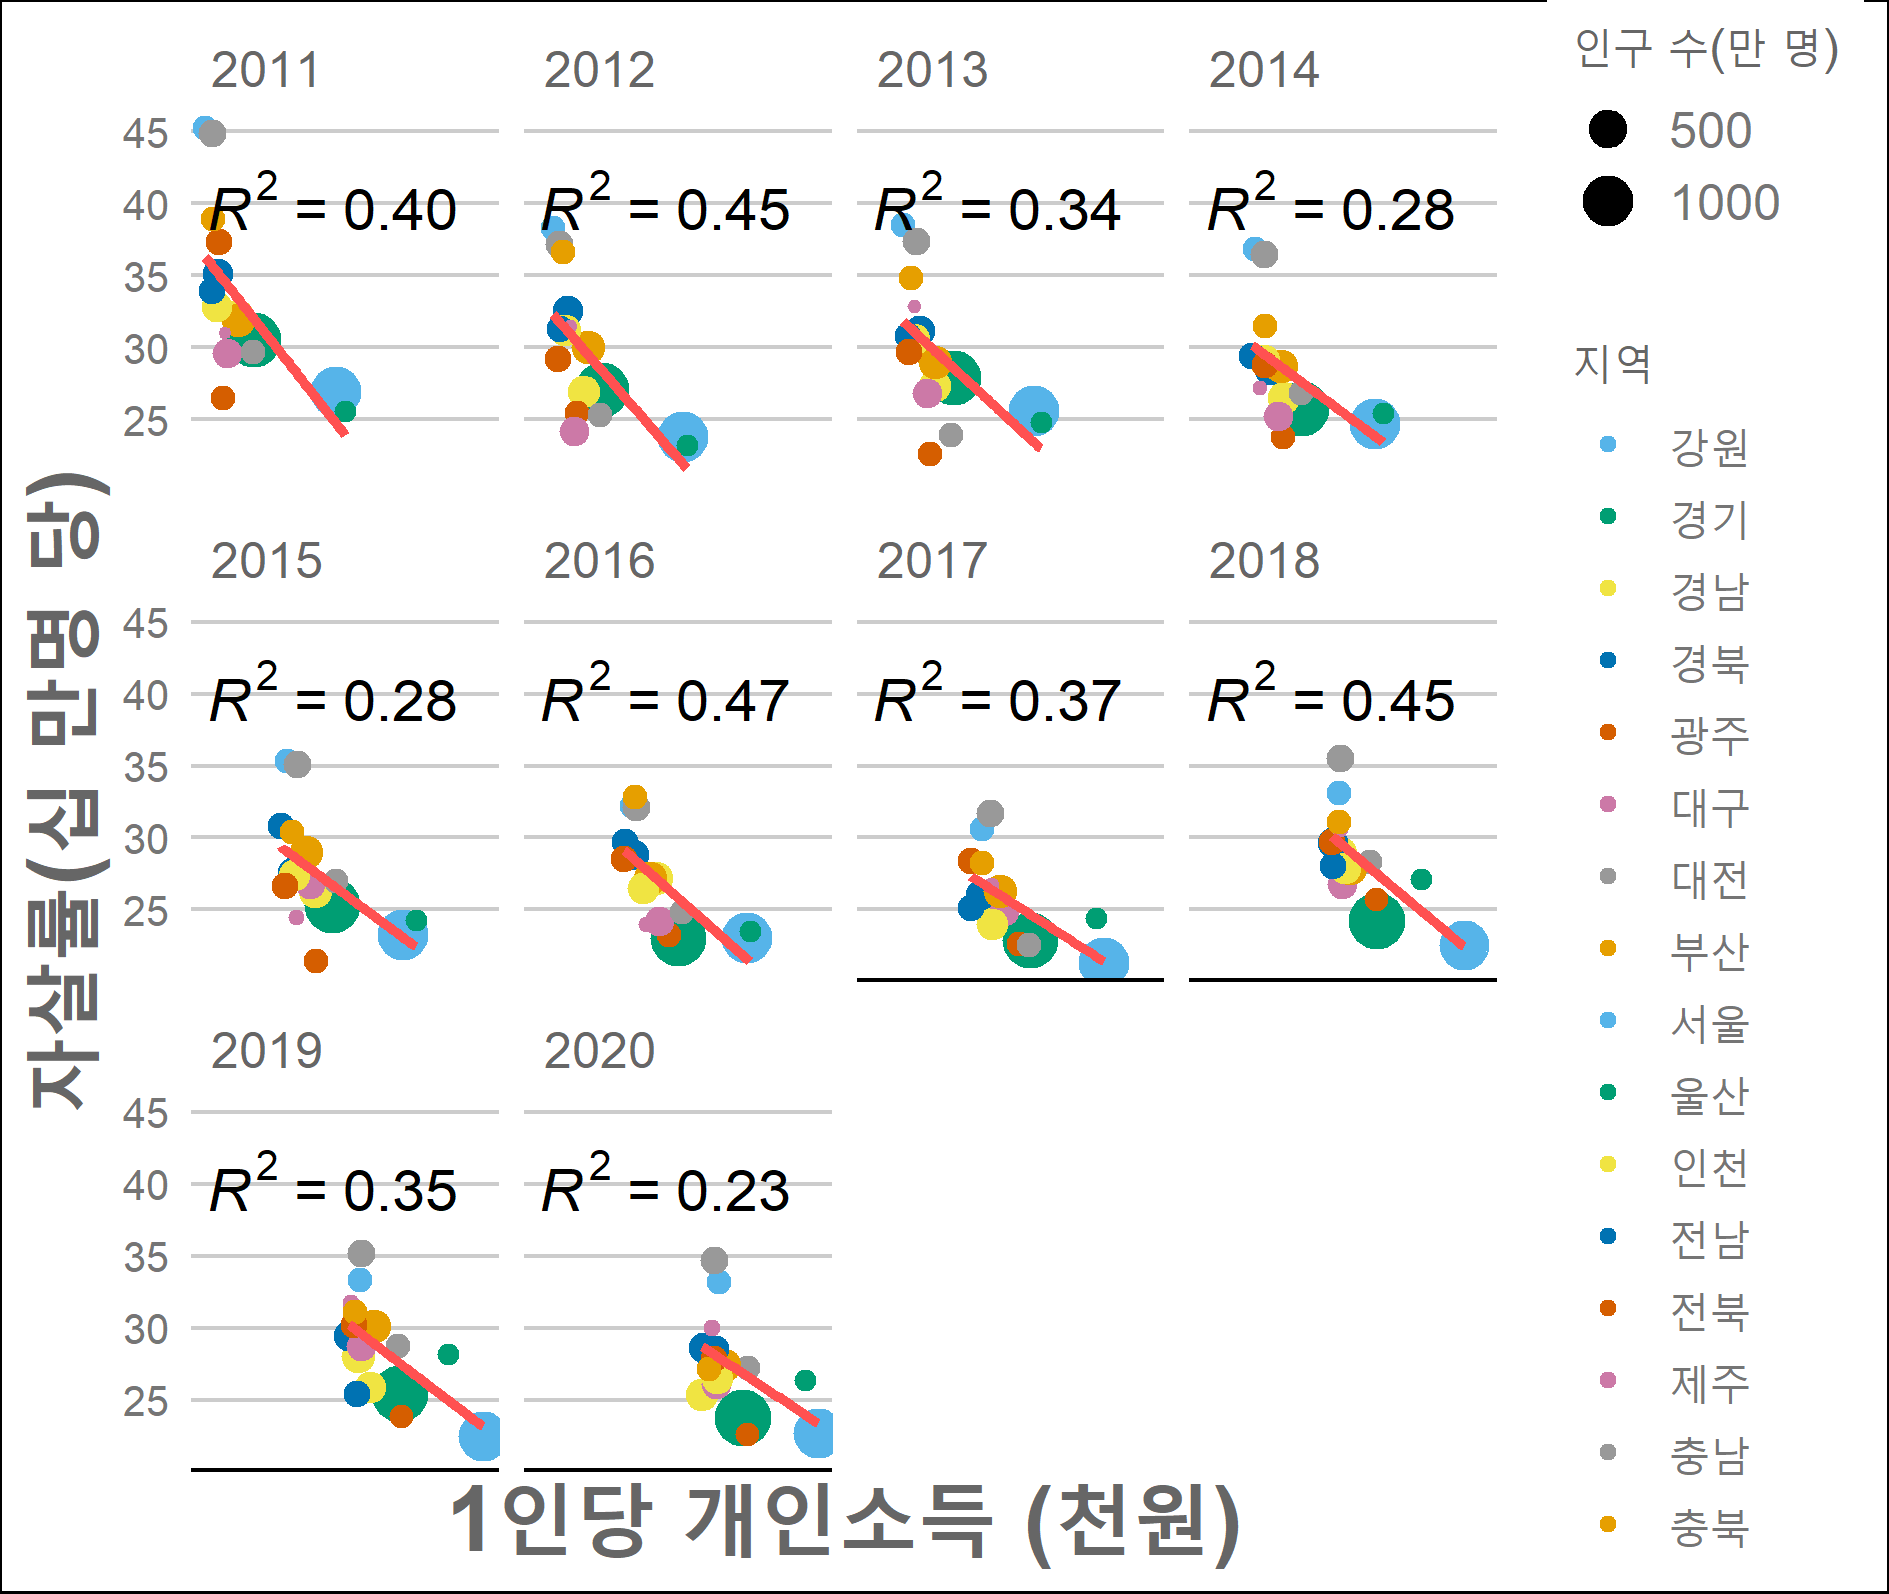
\includegraphics[height = 6cm, width = \linewidth]{c2.png}
        \caption{1인당 개인소득 - 자살률}
        \label{fig:pic151}
        \endminipage\hfill
    \end{figure}
    연도별로 각 변인과 자살률의 상관관계를 살펴봄으로써, 앞서 파악한 자살률과 각 변인과의 상관관계가 시기와는 무관하게
    유의미한 상관성을 나타내고 있는지 확인해보고자 했다. 
    
    최근 들어서 지역과 무관하게 기온이 전반적으로 상승하는 추세를 띄는 것에 비해,
    자살률은 전반적으로 낮아지는 양상을 띄고 있으므로 기온과 자살률 간의 상관관계가 줄어들고 있다고 판단하였다.(그림 11) 주민등록인구수와 자살률과의
    상관관계는 오히려 연도별로 증가하고 있다.(그림 12) 연도별로 각 지역의 주민등록인구수는 크게 차이가 없으며, 인구 수가 많은 수도권의 자살률은 비교적 낮은
    수준으로 유지된다는 점을 확인할 수 있다. 이러한 점에 비추어 보면, 최근 들어서 높아지는 $R^{2}$ 값은 인구와의 관계가 증가했다기
    보다는 수도권 외 지역의 전반적으로 자살률이 감소하여 상대적으로 자살률이 낮은 수준으로 유지되는 수도권과 비슷해지는 현상에 따라
    나타나는 부가적인 결과로 이해하였다. 또한 인구 수가 그 자체로 특질을 갖는 변수가 아니라는 점을 고려하였을 때, 인구 수와 자살률을 매개시키는 제 3의 변수가 존재할 가능성도 배제할 수 없다.
    이혼건수(그림 13)의 시기가 변함에 따라서 자살률과의 상관관계가 높아지는 것으로 확인되었으며,
    이는 이혼 비율 줄어듦에 따라 이혼으로 비롯되는 경제적문제나 정신적문제가 발생하게 되는 개인적 상황이 상대적으로 더 큰 영향을 미치게 되는 
    사회적 요소가 생겨나기 때문이라 판단하였다. 
    건강생활실천률이 가지는 주관적이고 개인적인 성질의 특성으로 인해서인지, 건강생활실천률은 연도와 무관하게 자살률과 꾸준한 상관성을 띄지 않았고
    2017년과 2018년에 $R^{2}$ 값이 높게 나오는 것을 확인할 수 있었다.(그림 14) 2017년에는 다른 년도에 비해 전반적으로 각 지역들의 자살률이 평균 근처에서 낮게 형성되었고, 
    2018년에는 다른 연도에 비해서 건강생활 실천률 자체가 높은데, 이와 같은 데이터의 특수성이 $R^{2}$ 값에 영향을 준 것으로 판단하였다. 
    모든 지역에 대해서 전체적으로 시간이 지남에 따라 1인당 개인소득은 증가하였다.(그림 15) 
    그와 함께 자살률도 감소하는 추세를 보였는데, 개인소득이 자살률과 직접적으로 연관을 가지는 것인지 자살률과 개인소득 사이를 매개하는
    다른 변인이 존재하는지는 파악하기 어려웠다. 자살률은 2020년 들어서 개인소득과 자살률의 $R^{2}$ 값이 낮아졌으며, 이 부분에 관련하여 추가적인 연구가 필요하다고
    판단하였다.
    \begin{figure}[!ht]
        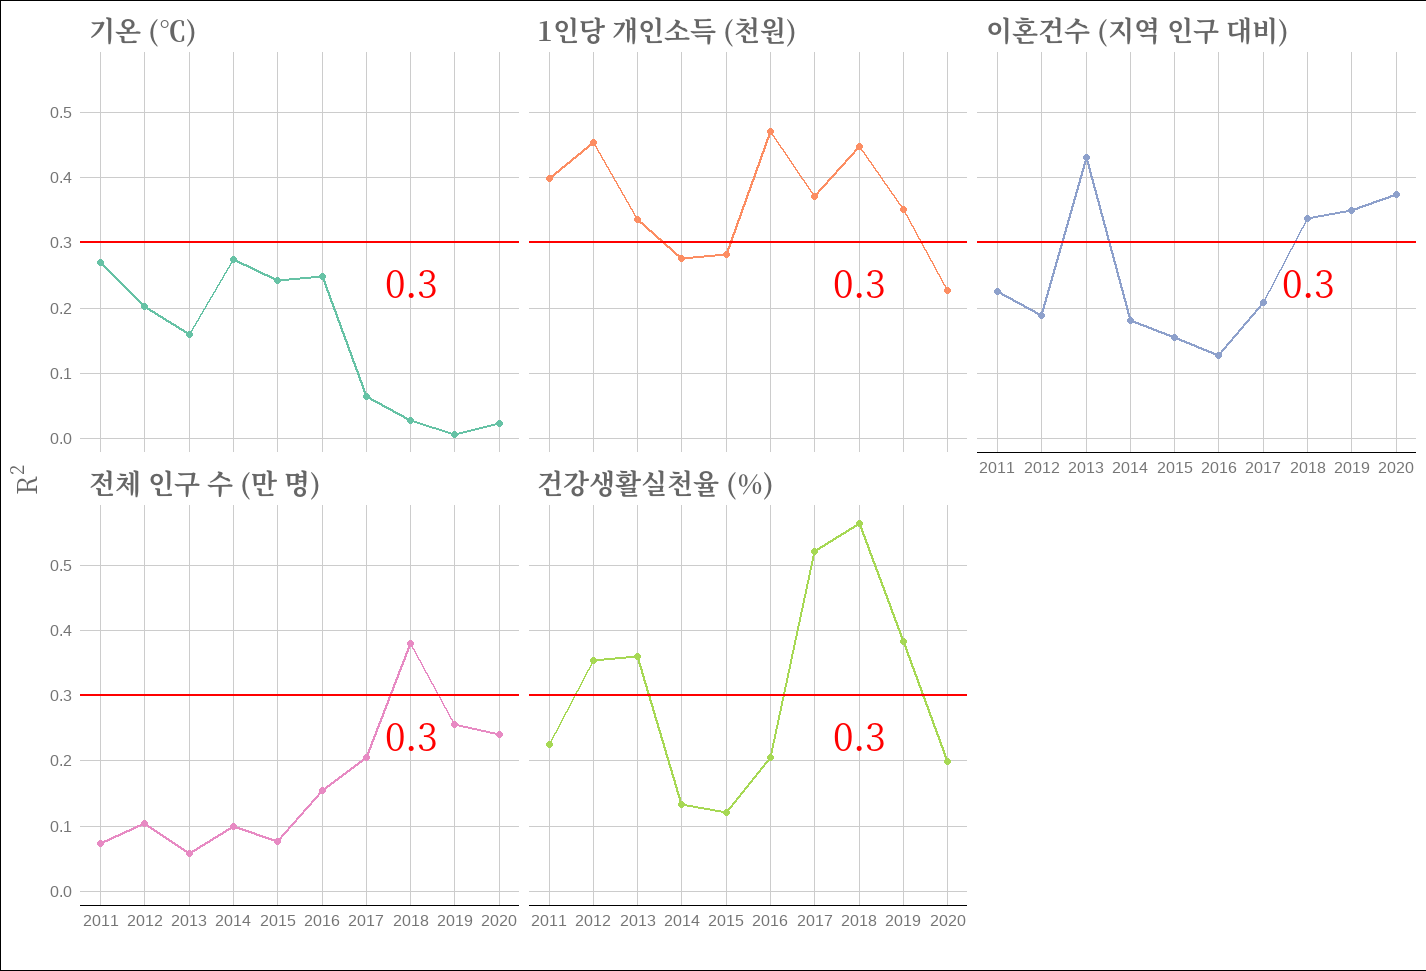
\includegraphics[width = 0.8\textwidth]{picture6.png}
        \caption{5개의 독립변인과 자살률의 연도별 $R^{2}$ 변화}
        \label{fig:pic6}
      \end{figure}
    
     앞선 논의에서는 $R^{2}$ 값의 연도별 변화를 추적함으로써 시기와 무관하게 꾸준히 자살률과 상관성이 높은 변인을 알아보고자 하였다. 이를 종합하며 (그림 17)에 나타내었다. 
    기온의 경우에는 2017년 – 2020 년 동안 자살률과의 
    연관성이 아주 크게 감소한 것으로 나타났고, 전국의 기후가 전반적으로 더워지는 상황 속에서 각 지역의 기후 편차가 적어짐에 따라 기온이 자살률의 차이를 설명하기 
    어려워지고 있다고 판단하였다. 건강생활실천률의 경우에는 주관성의 요소가 크기 때문인지 자살률과 상관성을 갖는 정도가 해마다 크게 변동하였다. 이혼 건수의 경우에도 건강생활실천률과
    비슷하게 개인적인 상황을 나타내기 때문인지 자살률과 상관성을 갖는 정도가 일관성이 존재하지는 않았다. 그러나 이혼건수의 경우 2018년부터 $R^{2}$ 값이 0.3 이상을 유지해오는 점은 
    이후 분석해볼 가치가 있어보인다. 1인당 개인소득은 앞서 살펴본 바와 같이 꾸준하게 0.3 이상의 $R^{2}$ 값을 유지해왔으며, 이를 바탕으로 자살률과 가장 높은
    상관관계를 갖는 변인이라 판단할 수 있었다. 그러나 2020년 들어 자살률과의 상관관계가 나타나고 있는 점으로 미루어 보아, 자살률에 영향을 미치는 요인으로서의 
    경제적 변인이 갖는 의미가 퇴색되고 있는 것인지 판단할 필요가 있다고 느꼈다.

    \section{결론}
    \subsection{정리}
    본 연구는 한국의 자살률이 높도록 만드는 변인을 찾아내고자, 국내 지역별 데이터를 활용해 자살률과 상관관계가 높은 요소를 판별하고자 
    하였다. 이를 통해서 경제적 변인(1인당 개인소득)이 자살률과 가장 높은 상관관계를 갖는다고 판단할 수 있었다. 그러나 2020년에는 기존에 
    존재하던 1인당 개인소득과 자살률의 상관관계가 약해진 것을 확인할 수 있었다. 과연 2020년 들어서 1인당 개인소득과 자살률의 약해진 상관관계가 2020년의 코로나 19
    전염병 사태와 관련해서 나타나는 일시적인 것인지, 혹은 본 연구에서 밝히지 못한 다른 변인과 관계되어서 유의미한 하락인지 연구해볼 가치가 있다고 
    생각한다. 그리고 앞서 살펴본 선행연구에서 유의미하게 자살률과 상관관계를 가질 수 있을 것이라고 판단한 정신적/건강적문제는, 본 연구에서는
    경제적 요인에 비해서 상대적으로 약한 상관관계를 띔을 파악할 수 있었다. 마지막으로 주민등록인구수의 경우 인구 수가 많은 수도권(서울, 경기)와 
    그 외 집단으로 나누어졌을 때, 인구 수가 특정 수준 이상으로 많아지면 자살률이 낮아지는 것을 발견할 수 있었지만 인구 수의 변이가 자살률에 
    직접전인 연관을 준다기 보다는 인구 수와 자살률을 매개하는 제 3의 변수가 있을 것이라 추측하였다. 
    \subsection{한계}
    
    본 연구의 분석에 대해 생각해볼 수 있는 한계점은 아래와 같다. 

    \begin{enumerate}
        \item 본 연구는 자살 현상의 원인을 지나치게 단순화해 파악하여, 각 독립 변인과 자살률의 1 대 1 상관관계 만을 파악하고 각 독립변인과
        자살률을 매개할 수 있는 혼동변수(confounding variable)의 존재를 간과했다.
        \item 선행연구를 통해 선정한 자살률과 관계 있는 네 가지 범주에 속하는 변인을 선정하는 것에 있어서 주관성이 개입되었다.
        \item 지역별 데이터를 사용하였으나 지역 별 특성을 나타낼 수 있는 사회문화적 가치에 대한 고려 없이 판단하여 각 독립 변인이
        자살률에 미치는 영향이 지역별로 다를 수 있을 가능성을 배제하였다.
        \item 본 연구에서 사용한 KOSIS 역별 e-지방지표 데이터의 한계로 인해 신체적/정신적 문제와 자살과의 연관성을 구체적으로 확인해보지 못했다.
        \item 유의수준을 0.05로 설정하여 연도별 데이터의 통계적 유의성을 판단하였을 때 3개 년도(2011년, 2014년, 2016년)만이 통계적으로 유의한 
        결과를 나타내었다. 비록 각 연도별 데이터의 표본이 16개 지역 밖에 되지 않아 p-value를 바탕으로 통계적 유의도를 측정하는 것이 
        부적절할 수 있다. 그러나 분석을 대상으로 삼은 2011년-2020년 중 3개 년도만이 통계적으로 유의미하다는 점은, 데이터를 분석한 결과가 각 독립변인과 자살률의 관계에 유의미한 시사점을 가져다 
        주지 못할 수 있음을 시사한다.  
    \end{enumerate}

    위의 한계점을 바탕으로 혼동변수를 찾고, 신체적/정신적 문제 또한 고려하며 지역별 특색을 반영할 수 있는 충분한 표본의 데이터가 확보될 수 있다면 
    자살률에 가장 큰 영향을 끼칠 수 있는 변인을 객관적으로 파악할 수 있을 것이다. 

    \pagebreak
    \section{References}
    이용재 \& 김경미. (2018). 한국의 지역별 자살률 변화와 요인 분석. 한국콘텐츠학회 논문지, 18(8), 51-61.\\
    김기원 \& 김한곤. (2011). 노인자살률에 영향을 미치는 요인에 대한 거시적 분석. 한국인구학, 34(3), 31-54.\\
    이민아 \& 강정한. (2014). 한국 사회 자살률의 변동과 원인: 지역단위 지표를 이용한 패널 분석. 한국인구학, 37(2), 1-19.\\
    한국생명존중희망재단, (2021). 5개년(’13~’17) 전국 자살사망 분석 보고서. 보건복지부:한국생명존중희망재단.\\
    한국생명존중희망재단, (2021). 2021 자살예방백서, 보건복지부:한국생명존중희망재단.\\
    박용주, (2021년 9월 28일). 한국 자살률 OECD 1위…20대 여성·10대 남성 크게 늘어. 연합뉴스.\\
    https://www.yna.co.kr/view/AKR20210928073600002\\
    노진섭, (2022년 5월 18일). 10년 새 자살률 100% 증가한 한국에 무슨 일이 있었나?. 시사저널. https://www.sisajournal.com/news/articleView.html?idxno=238338\\
    한해 사회경제적 질병부담 151조 원, 단일 원인 1위는 ‘자살’. KBS뉴스. (2019년 4월 10일). https://news.kbs.co.kr/news/view.do?ncd=4177583\\
    윤소영, \lbrack정신건강칼럼 : 3월\rbrack 가까운 사람의 자살로 인한 슬픔. 서울아산병원 정신건강의학과 정신건강이야기. https://amc.seoul.kr/asan/depts/psy/K/bbsDetail.do?menuId=862\&contentId=252509















\end{document}